\documentclass[12pt]{book}
\usepackage[margin=2cm]{geometry} 
\usepackage{amsmath,amssymb,amsthm}
\usepackage[noend]{algpseudocode}
\usepackage[dvipsnames]{xcolor}
\usepackage{color,soul}
\usepackage{hyperref}
\usepackage{imakeidx}
\usepackage{beton}
\usepackage{concmath}
\usepackage{breqn}
\usepackage{algorithm}
\usepackage{float}
\usepackage{graphicx}
\usepackage{wrapfig}
\usepackage{epigraph} 
\usepackage{lastpage}
\usepackage{fancyhdr}
\pagestyle{fancy}
\fancyhf{}
\fancyfoot[C]{\thepage}
\rhead{cleopinoli 2024}
\lhead{Internet, Reti e Sicurezza}
\makeindex[columns=2, title=Indice Alfabetico dei Contenuti]

\newcommand{\openapex}{``}





\title{Internet, Reti e Sicurezza\\Digital Ed.}
\author{cleopinoli}
\date{}

\begin{document}

\maketitle
\pagenumbering{roman}
\tableofcontents
\newpage
\pagenumbering{arabic}
\setcounter{page}{1}
\addcontentsline{toc}{chapter}{Introduzione}
\chapter*{\begin{center}\texttt{Introduzione}\end{center}}
\hrulefill \\
\addcontentsline{toc}{section}{Cos'è Internet?}
\section*{\textcolor{Blue}{Cos'è Internet?}}
\index{Internet} Fondamentalmente è una rete che collega tra loro più unità di calcolo sparse geograficamente. Si tratta di una \index{rete!a comm. di Pacchetto}rete a commutazione di pacchetto (packet-switch network, PSN), in cui più terminali \index{host}\index{End System}(o End System, o Host, insomma qualsiasi tipo di computer che si trova ad un capo estremo della rete, un laptop, uno smartphone, un sensore...) condividono lo stesso cammino di rete o una parte di esso. Torneremo su commutazione di circuito e di pacchetto a breve.\\


 \noindent Normalmente, i terminali non sono collegati tra loro in modo diretto, ma tramite dispositivi di commutazione e instradamento (router)\index{router} che prelevano le informazioni in dei pacchetti e le inoltrano sui link di uscita. Il percorso compiuto dai pacchetti attraverso la rete prende il nome di Route\index{route}, o Path. Letteralmente \textit{percorso}.\\

 \noindent L'accesso dei terminali ad Internet avviene attraverso gli ISP\index{ISP} (Internet Service Provider), aziende di telecomunicazioni come AT\&T o Vodafone, che costuiscono ciascuna una rete di router a cui poter collegare gli access point come la ADSL domestica (che di per sé costituisce una rete, in questo caso domestica, in cui tutti gli Host comunicano tra loro (internamente) e con il resto di internet (esternamente) attraverso quello che comunemente chiamiamo \index{modem}Modem o \index{gateway}Gateway).\\

 \noindent  TCP/IP: insieme di protocolli (spesso si parla di stack TCP/IP, perché sono posti uno sopra l'altro) che gestiscono invio e ricezione di pacchetti in rete.\\

 \noindent \index{intranet}Intranet: è un tipo di rete privata, strutturata similmente alla pubblica Internet.\\

 \noindent \index{protocollo}Protocollo: insieme di regole formalmente descritte al fine di favorire la comunicazione tra una o più entità (è un termine generico che si può applicare anche ad altri contesti, ovviamente in questo caso parliamo di Host o di componenti in grado di comunicare in rete).\\

 \noindent App distribuite: in Internet si lavora tramite app distribuite, i.e. due o più processi che vengono eseguiti in parallelo su macchine diverse e che interagiscono tra loro attraverso Internet. \\

 \noindent Host: termine che si riferisce a dei sistemi periferici che ospitano programmi applicativi come ad esempio web browser; Gli host si suddividono ulteriormente in Client e Server, rispettivamente host che richiedono un serivizio e quelli che lo forniscono. Un singolo host può fungere da client e da server (connessione Peer-to-Peer). \\

\noindent \index{DSL}DSL (Digital Subscriber Line): accesso residenziale a banda larga. \\ 


\addcontentsline{toc}{section}{Stack dei layer di Internet}
\section*{Stack dei layer di Internet: TCP/IP VS modello ISO/OSI}
\index{TCP/IP, stack}\index{ISO/OSI, modello}
\begin{table}[h]
\begin{tabular}{|ll|ll|l}
\cline{1-4}
\multicolumn{2}{|l|}{TCP/IP}            & \multicolumn{2}{l|}{ISO/OSI}                                                                                                                             &                                                                                                      \\ \hline
\multicolumn{1}{|l|}{Layer}        & n° & \multicolumn{1}{l|}{Layer}                                                                           & n°                                                & \multicolumn{1}{l|}{Esempi di Protocolli}                                                            \\ \hline
\multicolumn{1}{|l|}{Applicazione} & 5  & \multicolumn{1}{l|}{\begin{tabular}[c]{@{}l@{}}Applicazione\\ Presentazione\\ Sessione\end{tabular}} & \begin{tabular}[c]{@{}l@{}}7\\ 6\\ 5\end{tabular} & \multicolumn{1}{l|}{\begin{tabular}[c]{@{}l@{}}HTTP(S), POP, SMTP,\\ FTP, SSH, DHCP...\end{tabular}} \\ \hline
\multicolumn{1}{|l|}{Trasporto}    & 4  & \multicolumn{1}{l|}{Trasporto}                                                                       & 4                                                 & \multicolumn{1}{l|}{TCP, UDP}                                                                        \\ \hline
\multicolumn{1}{|l|}{Rete}         & 3  & \multicolumn{1}{l|}{Rete}                                                                            & 3                                                 & \multicolumn{1}{l|}{IPv4, IPv6, ICMP}                                                                      \\ \hline
\multicolumn{1}{|l|}{Datalink}     & 2  & \multicolumn{1}{l|}{Datalink}                                                                        & 2                                                 & \multicolumn{1}{l|}{MAC}                                                                             \\ \hline
\multicolumn{1}{|l|}{Fisico}       & 1  & \multicolumn{1}{l|}{Fisico}                                                                          & 1                                                 & \multicolumn{1}{l|}{Ethernet, cavo coassiale}                                                        \\ \hline
\end{tabular}
\end{table}

 \noindent Sono due rappresentazioni della stessa stack di classi di protocolli, semplicemente l'ISO\footnote{International Standardization Organization, l'agenzia che si occupa di distribuire standard di varie tecnologie e produzioni.} ha separato l'application layer in 3 layers (Application, Presentation, Session), che è una rappresentazione un po' più dettagliata, ma noi faremo riferimento principalmente al modello TCP/IP. (N.B.: alle volte, nel modello TCP/IP, i layer Datalink e Fisico\footnote{il layer fisico/physical alle volte viene detto anche Network Access Layer.} vengono trattati indistintamente, come fossero un layer unico.) \\

\addcontentsline{toc}{section}{Tipi di ritardo e altri concetti}
\section*{Tipi di ritardo e altri concetti}\index{ritardi}
\noindent Tipi di ritardo (accenno, ci torneremo)\footnote{in verità quasi tutto questo capitolo è un accenno a cose che vedremo più avanti in maggiore dettaglio, ndr.} 
\begin{itemize}
    \item [i.] di Elaborazione: si crea nel router per esaminare il pacchetto;
    \item [ii.] di Accodamento: si crea in coda in uscita, un buffer;
    \item [iii.] di Trasmissione $(=\dfrac{L}{R})$: dipende dalla dimensione del pacchetto (L);
    \item[iv.] di Propagazione: prettamente fisico, dipende dalla distanza tra router A e router B.
\end{itemize}

\noindent La somma di questi ritardi costituisce il \index{delay, nodal}nodal delay, il ritardo accumulato ad ogni nodo del percorso. \\

\noindent \index{network!core}\index{network!edge}Network core vs Network edge: fondamentalmente il network edge sono i sistemi periferici (host come laptops o smartphones), mentre il network core è la struttura che li collega (routers etc.). \\

\noindent \index{LAN}LAN (Local Area Network): usata per collegare end systems ad un edge router. La tecnologia d'accesso usata di solito in queste reti è \index{Ethernet}Ethernet. \\

\noindent Standard IEEE che regolamenta il \index{Wi-Fi}Wi-Fi\footnote{Secondo la Wi-Fi Alliance, il termine ``Wi-Fi'' non è mai stato la contrazione di ``\underline{Wi}reless \underline{Fi}delity, sebbene l'IEEE affermi diversamente.}: 802.11. \\

\noindent Qualche nota sui Physical Media (Mezzi di trasmissione fisici, i.e. cavi eccetera):
\begin{itemize}
    \item Twisted Pair Copper wire (il doppino intrecciato in rame)\index{doppino, in rame}:
    \begin{itemize}
        \item UTP\index{UTP} (Unshielded Twisted Pair, doppino non schermato): usato comunemente nelle LAN. Un cavo UTP di categoria 6A può trasmettere ad una velocità fino a 10Gbps;
        \item La ragione per cui i fili nel doppino sono intrecciati a due a due a quella maniera ha a che fare con la cancellazione dei disturbi del segnale;
    \end{itemize}
    \item Cavo coassiale\index{coassiale, cavo}: quello a sezione circolare dell'antenna TV. Può essere usato in contemporanea da più end systems; alcune categorie trasmettono a velocità nell'ordine di diversi Gbps;
    \item Fibra ottica\index{fibra ottica}: molto veloce, molto costosa, va dai 51.8M ai 39.8 Gbps;
\end{itemize}

\noindent \index{tempo di trasmissione}Il tempo di trasmissione è dato da $\dfrac{L}{R}$, dove L = dimensione del pacchetto in bit e R = transmission rate sul link.\\

\noindent \index{Store-and-Forward}Store-and-forward: il router deve ricevere tutto il pacchetto prima di inoltrarlo dove opportuno; così facendo, il ritardo totale diventa $=\dfrac{2L}{R}$ (per ciascun nodo, credo).\\

\noindent \index{modem}``Modem'' sta per \underline{Mo}dulatore-\underline{Dem}odulatore: sebbene spesso ci riferiamo allo ``scatolotto'' che collega la nostra LAN domestica ad Internet con il termine Modem (quei dispositivi come il TIM Hub, insomma, a volte li si chiama anche Router, che non è troppo sbagliato), in realtà il modem è un modulo incluso in quello scatolotto.\\

\noindent \index{rete!a comm. di Pacchetto}Commutazione di Circuito vs Commutazione di Pacchetto\index{rete!a comm. di Circuito}:
\begin{itemize}
    \item Comm. di circuito: le risorse richieste da un end system per comunicare sono riservate ad esso per tutta la durata della connessione; è il caso della telefonia, se qualcuno sta usando il telefono di casa in una stanza, un secondo telefono collegato alla stessa linea non può avviare un'altra chiamata);
    \item Comm. di pacchetto: le risorse non sono riservate, ma più end systems usano il canale più la banda viene limitata a ciascuno;
\end{itemize}

\noindent La commutazione di circuito può avere due tipi di multiplexing\index{multiplexing}: Frequency-division e Time-division:

\begin{figure} [h]
    \centering
    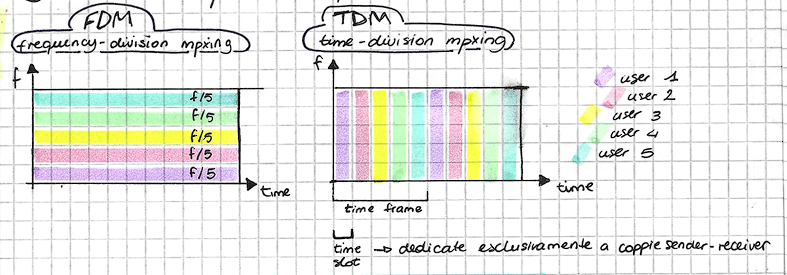
\includegraphics[width=0.6\linewidth]{Figures/01/circswitch.png}
    \label{fig:circswitch}
\end{figure}

\begin{figure}
    \centering
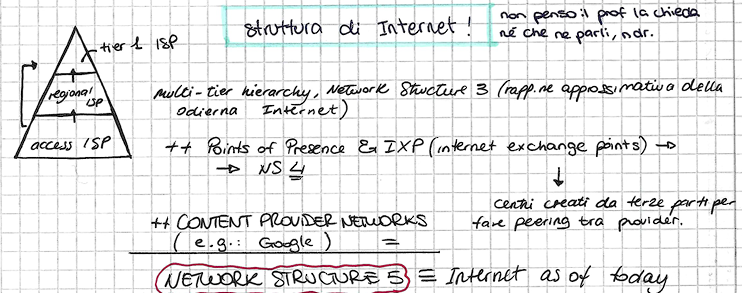
\includegraphics[width=0.8\linewidth]{Figures/01/isp-hierarchy.png}
    \caption{Sì non credo vi verrà richiesta, ma nel dubbio è una cosa del genere.}
    \label{fig:in-structure}
\end{figure}

\noindent In Fig. \ref{fig:in-structure} è riassunta la struttura di Internet e le sue evoluzioni con le varie addizioni di elementi come i Point of Presence \& IXP.\\

\noindent \index{intensità di traffico}Intensità di traffico: $\dfrac{L\cdot a}{R}$, L e R li abbiamo già menzionati, $a=$ average rate of packets per second; un'intensità di traffico $>1$ equivale a dire che la $\#$ di bit che arriva in coda supera la $\#$ di bit che esce dalla coda (converrete con me che è una cosa da evitare, significa che la roba che entra supera la roba che esce, c'è congestione).\\


\begin{wrapfigure}{r}{0.4\textwidth}
 \begin{center}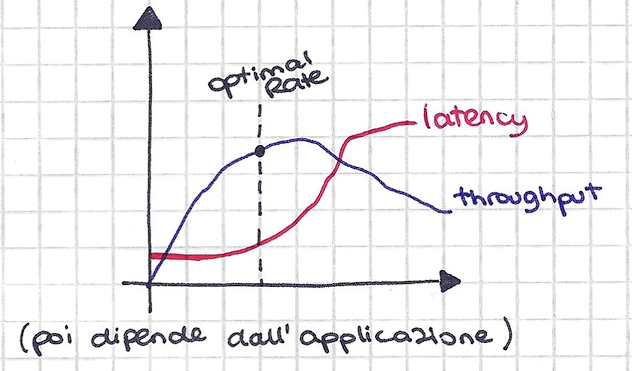
\includegraphics[width=1\linewidth]{Figures//01/optrate.png}
  \end{center}
\end{wrapfigure}
\newpage

\noindent \index{latenza}Latenza: intervallo di tempo tra quando spedisco un input e quando è disponibile l'output.\\

\noindent \index{throughput}Throughput: ``vera velocità'' di rete, vera capacità di un canale trasmissivo. Non si può considerare costante, si parla solo di throughput medio end-to-end.\\

\noindent \index{bandwidth}Bandwidth: intervallo di frequenza che un sistema può garantire per trasmettere. \index{bitrate}Bitrate: dipende dalla bandwidth (teorema di Nyquist-Shannon)\index{teorema!di Shannon}\index{teorema!di Nyquist} (garantito nominalmente).

\begin{figure} [h]
    \centering
    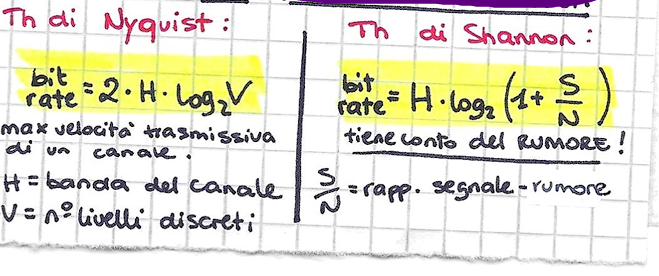
\includegraphics[width=0.5\linewidth]{Figures//01/shannon-nyquist.png}
\end{figure}

\begin{wrapfigure}{l}{0.3\textwidth}
 \begin{center}
 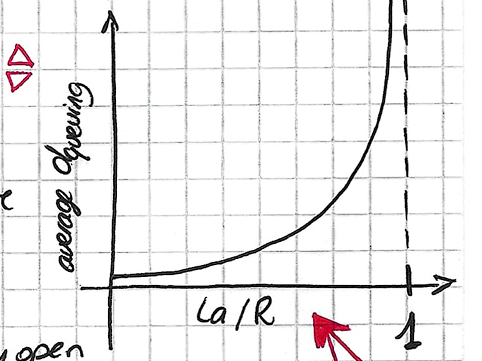
\includegraphics[width=1\linewidth]{Figures/01/laR.png}
  \end{center}
\end{wrapfigure}
\noindent Intensità di traffico: $\dfrac{L\cdot a}{R}$, L e R li abbiamo già menzionati, $a=$ average rate of packets per second; un'intensità di traffico $>1$ equivale a dire che la $\#$ di bit che arriva in coda supera la $\#$ di bit che esce dalla coda (converrete con me che è una cosa da evitare, significa che la roba che entra supera la roba che esce, c'è congestione).\\

\noindent Note sugli attacchi DoS (Denial of Service)\index{attacco!Denial of Service}:
\begin{itemize}
    \item vulnerability attack: usa un messaggio ``maligno'' per compromettere app o host;
\end{itemize}

\begin{itemize}
    \item bandwidth flooding\index{attacco!bandwidth flooding}: invio smisurato di pacchetti al target allo scopo di congestionare l'access link e renderlo inutilizzabile;
    \item \index{attacco!connection flooding}connection flooding: richiesta elevata di connessioni TCP fully open (che rimangono sempre attive) al punto tale che l'host vittima non riesce più ad accettarne altre genuine. Spesso questo attacco è reso possibile grazie a Distributed DoS\index{attacco!DDoS}, i.e. l'attacker controlla più macchine ``zombie''  che dirotta a sua discrezione all'attacco della vittima.
\end{itemize}

\noindent \index{packet sniffing}Packet sniffing (che è quello che fa Wireshark): i bad guys si posizionano tra due host e ``origliano'' il traffico senza manometterlo allo scopo di estrarre informazioni sensibili;

\noindent \index{attacco!IP spoofing}IP spoofing: ``rubare'' l'identità di qualcun altro mediante il suo indirizzo IP;

\noindent \index{traceroute}Traceroute: manda tot pacchetti ai router compresi tra host e destinazione, rilevandoli tutti
\begin{verbatim}
    tracert www.rai.it (212.162.68.64)
\end{verbatim}

\noindent Ogni protocollo appartiene ad un qualche layer della stack e può essere hardware, software o misto.\\

\noindent \index{PDU}PDU (Protocol Data Unit): l'unità di messaggio, che a seconda del layer in cui si trova prende un nome diverso (e.g.: frame, datagramma). La PDU è sempre formata da un header (detto anche PCI o Protocol Control Information) e da un payload (detto anche SDU o Service Data Unit), dove header contiene informazioni per la trasmissione e il payload è il contenuto del messaggio (il payload è generalmente ottenuto dalle PDU dei livelli più alti);

\noindent \index{incapsulamento}Incapsulamento: ciascun layer riceve il messaggio dal layer sopra, aggiunge un suo header, passa il nuovo messaggio al layer sotto. Nel layer sotto succede di nuovo: il layer riceve questo (header + payload) e lo considera come un payload', aggiunge il suo header e passa header' + payload' ancora sotto;\\

\noindent \index{SAP}SAP Service Access Point: servizi messi a disposizione dalle interfacce che si trovano tra due layer comunicanti della stack.\\

\noindent Per fornire accesso a Internet agli utenti, gli ISP distribuiscono lungo il territorio dei PoP, Points of Presence.\\

\noindent Indirizzi della forma $192.168.1.\#\#\#$ non sono indirizzi pubblici, ma interni alla nostra rete.\\

\noindent

\noindent Fiber To The...

\begin{itemize}
    \item FTTH: ...Home
    \item FTTN: ...Node
    \item FTTC: ...Cabinet
    \item FTTS: ...Street (=FTTC)
    \item FTTB: ...Building
\end{itemize}

\noindent \index{best effort}Internet ha un generale approccio al servizio detto ``best effort'' (i.e.: ``che Dio ce la mandi buona''): nulla è di fatto garantito al 100\%, ma tutti fanno del proprio meglio perché funzioni.\\
\newpage
\noindent \index{legge!di Metcalfe}\textcolor{Blue}{Legge di Metcalfe (che allego qui ma non vi serve): ``L'utilità e il valore di una rete sono proporzionali al quadrato del nr di utenti.'' Dato il nr di utenti, il massimo numero di connessioni possibili è $= n^2 - n$. (Si tratta di una legge di dubbia correttezza e largamente contestata, oltre al fatto che non è mai stato possibile testarla con dati reali).}\\

\noindent \textcolor{Blue}{LO! Story Time: La prima parola ad essere trasmessa in una versione preistorica di Internet è stata: \texttt{`LO'}. Transitava dal UCLA al SRI e doveva finire per essere la parola ``LOGIN'', lettera dopo lettera, ma per qualche ragione l'host del SRI crashò ricevendo la G. L'ingegnere Leonard Kleinrock, che era lì a lavorare al progetto ARPANET, scrisse in una celebre intervista che quel tentativo fallito di trasmettere la parola in rete ebbe comunque qualcosa di \textit{profetico:} ``Lo'', come in ``Lo and behold!'' (che più o meno significa \textit{``Ecco, preparatevi!''}), come a presagire la svolta enorme che sarebbe arrivata in futuro dopo quell'esperimento - con la nascita di Internet.}
\newpage
\addcontentsline{toc}{chapter}{Application Layer}
\chapter*{\begin{center}Application Layer\end{center}}
\begin{center}(Layer 5 nello stack TCP/IP)\end{center}\hrulefill \\
\hrulefill \\
\addcontentsline{toc}{section}{Introduzione}
\section*{Introduzione}
Ci sono 2 principali architetture in cui gli host si dividono:
\begin{itemize}
    \item Client-Server (e.g.: web server);
    \item Peer-to-Peer;
\end{itemize}

\noindent Network application: coppia di processi che si scambiano messaggi.\\

\begin{figure} [h]
    \centering
    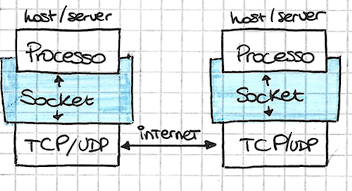
\includegraphics[width=0.5\linewidth]{Figures//02/netapps.png}
    \caption{Network application. Le \index{socket}socket (o API) sono interfacce software tra l'application layer e il transport layer di ciascun host. Ne esistono tra tutte le coppie di layer adiacenti.}
    \label{fig:enter-label}
\end{figure}

 \noindent Per identificare il processo ricevente serve specificare: l'indirizzo IP del Host, e un numero di porta\index{porta!numero di} che è dedicato al servizio (in maniera permanente o temporanea), tipo 100.100.100.1:80; ci sono diversi numeri di porta noti per essere riservati a certi servizi, tipo 80 è una porta riservata ad HTTP, 443 ad HTTPS, oppure 110 a POP3, 20 e 21 a FTP (dati e controllo rispettivamente), 67 e 68 a DHCP (requests e replies rispettivamente), 25 al mail server SMTP, 520 a RIP, e così via.\footnote{I numeri di porta sono documentati alla pagina: https://www.iana.org/assignments/service-names-port-numbers/service-names-port-numbers.xhtml}

\noindent La nostra app, a livello sottostante (transport layer), potrà usare principalmente due protocolli:
\begin{itemize}
    \item TCP (Transmission Control Protocol)\index{TCP}
    \begin{itemize}
        \item servizio orientato alla connessione (è richiesto che le parti comunicanti si identifichino e completino un handshake per iniziare a comunicare);
        \item trasferimento dati affidabile (gestione della perdita di pacchetti);
        \item HTTP, SMTP, FTP, HTTP 1.1, HTTPS, Telnet etc. si appoggiano tutti su TCP per il trasporto
    \end{itemize}
    \item UDP (User Datagram Protocol)\index{UDP}
    \begin{itemize}
        \item minimale, leggero, trasmette il minimo indispensabile delle informazioni necessarie per consegnare un pacchetto da punto A a punto B;
        \item connectionless: niente handshake, niente connessione preliminare tra A e B. Il messaggio viene sparato da A e se arriva o meno non è dato saperlo.
        \item per via della sua leggerezza, UDP alle volte viene utilizzato per lo streaming live e on-demand (e.g.: Twitch),  servizi per cui non è necessario garantire che tutti i dati arrivino a destinazione (al limite si perde qualche frame, ma il contenuto si capisce ancora abbastanza bene). 
    \end{itemize}
\end{itemize}

\begin{figure}[h]
    \centering
    
\includegraphics[width=0.5\linewidth]{Figures/02/tcp-udp.png}
    \caption{Non so a chi attribuire questa creazione, ma è uno dei miei esempi umoristici preferiti riguardo TCP vs UDP. Kudos al creatore originale.}
\end{figure}

\noindent Nessuno dei due implementa sistemi di crittografia, a meno che non si usi TCP con TLS (Transport Layer Security), ma di base TCP non fornisce questo servizio.\\

\addcontentsline{toc}{section}{HTTP}
\section*{\textcolor{RoyalBlue}{HTTP}} 
\index{HTTP}
\noindent \textcolor{RoyalBlue}{H}yper \textcolor{RoyalBlue}{T}ext \textcolor{RoyalBlue}{T}ransfer \textcolor{RoyalBlue}{P}rotocol, default port: 80\\

\noindent Protocollo a livello di applicazione \underline{Web}: una \index{web!pagina}pagina Web è un insieme di oggetti (e.g.: file HTML\footnote{Hyper Text Markup Language}, immagine JPEG, file JavaScript, file CSS...). Tipicamente alla base delle pagine Web c'è un file HTML di base, che fa riferimento agli altri oggetti della pagina attraverso i relativi \index{URL}URL\footnote{Uniform Resource Locator}.\\

\noindent I \index{web!browser}Web Browser (e.g.: Google Chrome) implementano il lato Client di HTTP;

\noindent È un protocollo stateless: se un client manda due richieste identiche nell'arco di qualche secondo, HTTP non ne ha alcuna memoria, risponderà 2 volte con la stessa risposta.

\noindent Connessioni TCP:
\begin{itemize}
    \item persistente: tutte le richieste/risposte avvengono nella stessa sessione TCP;
    \item non persistente: ogni richiesta/risposta avviene in una sessione TCP nuova a se stante (ogni volta ne viene avviata una nuova).
\end{itemize}
\noindent HTTP usa una connessione persistente di default, ma può usarle entrambe. \\

\noindent \index{round trip time}RTT - Round Trip Time: tempo impiegato da un pacchetto per andare da client a server e poi tornare indietro.

\begin{table}[h]
\centering
\begin{tabular}{|ll|}
\hline
\multicolumn{2}{|c|}{Messaggi HTTP} \\ \hline
\multicolumn{1}{|c|}{Richiesta} & \multicolumn{1}{c|}{Risposta}\\ \hline
\multicolumn{1}{|l|}{\begin{tabular}[c]{@{}l@{}}get$^1$ /dir/page.html$^2$ HTTP/1.1$^3$\\ $^1$Request line - metodo $^2$ URL $^3$ versione HTTP\end{tabular}}    & \begin{tabular}[c]{@{}l@{}}HTTP/1.1 200 OK$^4$\\ $^4$stato\end{tabular}            \\ \hline
\multicolumn{1}{|l|}{\begin{tabular}[c]{@{}l@{}}Header:\\ host: www.(...) \\ connection: close \textbackslash{}textit\{(non persistente)\}\\ user\_agent: Mozilla/5.0 (tipo browser)\\ ... *altre istruzioni HTTP*\end{tabular}} & \begin{tabular}[c]{@{}l@{}}Header:\\ connection: close\\ date:[current date]\\ server: Apache/2.2.3\\ last-modified: {[}date{]}\\ Content length: 6821 {[}byte{]}\\ Content type: text/html\\ *RIGA VUOTA, fine Header*\\ Contenuto: data data data...\end{tabular} \\ \hline
\end{tabular}
\end{table}

\noindent Qual è la differenza tra HTTP 1.0 e HTTP 1.1? La più importante forse è la persistenza della connessione (abbiamo visto cosa significa poco fa), oltre ad altre cose come, ad esempio, l'introduzione di meccaniche di caching.

\addcontentsline{toc}{subsection}{Cookies}
\subsection*{\textcolor{RawSienna}{Cookies}}
\index{cookies}


\noindent (argomento interno ad HTTP) I cookies sono un tipo di informazione che viene memorizzata lato client. Può servire in un secondo momento al server per ristabilire una connessione.

\begin{figure} [h]
    \centering
    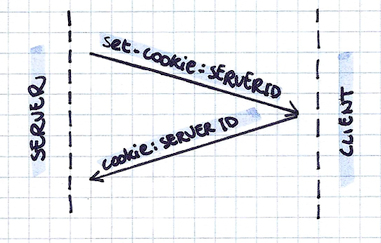
\includegraphics[width=0.6\linewidth]{Figures/02/cookies.png}
\end{figure}
\begin{itemize}
    \item ogni browser/sistema operativo archivia i cookies in un posto a sua discrezione, non esiste una convenzione universale su dove salvare i file di cookies;
    \item inizialmente, tutti i cookies erano semplici file di testo, ora la maggior parte è in formato SQLite (piccoli database!);
    \item non tutti i siti web usano i cookies;
    \item (tecnicamente,) i cookies sono \underline{facoltativi.}
    \item i cookies possono essere disabilitati;
    \item i cookies sono una minaccia per la privacy in quanto profilano gli utenti! Raccogliendo informazioni sulle loro abitudini, comportamenti etc. Vengono usati in quella che si dice Pubblicità comportamentale: analisi dell'attività in rete degli utenti al fine di permettere alle aziente di presentare a ciascuno pubblicità mirate ai loro gusti.\footnote{https://youronlinechoices.com/it/}
\end{itemize}


\addcontentsline{toc}{section}{Web Caching}
\section*{\textcolor{Brown}{Web Caching}}
\index{web!cache}\index{proxy server}
\noindent (o Proxy Server)\\

\noindent È un'entità della rete in grado di rispondere ad alcune richieste HTTP al posto dei server a cui sono indirizzate. Funziona circa così:
\begin{enumerate}
    \item Browser invia richiesta HTTP al proxy per (ad esempio) una pagina web;
    \item [2a] Se il Proxy contiene una copia in locale della pagina richiesta $\rightarrow$ il Proxy risponde al client;
    \item [2b] Se il Proxy non contiene una copia della pagina $\rightarrow$ il proxy richiede la pagina al server che dovrebbe averla, una volta che la ha ricevuta la recapita al client browser e ne salva una copia in locale. 
\end{enumerate}

\noindent ``Conditional GET'',\index{GET!conditional} richiesta dal proxy per il server: se l'oggetto richiesto è stato modificato di recente, mandamene la copia aggiornata, altrimenti manderò al client quella che ho io.\\

\noindent Perché si fa questo lavoro di web cache?
\begin{itemize}
    \item per ridurre i tempi di attesa\footnote{normalmente l'intensità di traffico è molto più alta al di fuori di una LAN (in uscita verso Internet) che non al suo interno, da cui le potenziali latenze elevate.};
    \item ridurre il traffico complessivo nel Web.
\end{itemize}
\noindent L'intensità del traffico\index{intensità di traffico} può essere misurata come: 
\[T = X \cdot \dfrac{Y}{Z}\]
dove:\\
$X=$ richieste/secondo;\\
$Y=$ Megabit/richiesta;\\
$Z=$ Megabit/secondo.\\


%%%%%%%%%%%%%%%%%%%%%%%%%%%%%%%%%%%%%%%%%%%%
%%%%%%%%%%%%%%%%%%%%%%%%%%%%%%%%%%%%%%%%%%%%

\addcontentsline{toc}{section}{Posta Elettronica}
\section*{\textcolor{Periwinkle}{e-Mail}}
\index{posta elettronica}
\noindent Componenti chiave del sistema di mailing in Internet:
\begin{itemize}
    \item User Agents\index{user agent}: lo strumento con cui si leggono/scrivono le mail, come la app di Gmail per Android o un browser web che accede al sito \hyperlink{mail.google.com}{https://mail.google.com/mail/};
    \item Mail Servers\index{mail!server}: il ``core'' dell'infrastruttura di e-mailing. È il mail server che contiene le caselle degli utenti, i messaggi viaggiano dal MS del mittente alla mailbox nel MS del destinatario/i;
    \item SMTP\index{SMTP} (Simple Mail Transfer Protocol): il principale protocollo a livello applicativo per la posta elettronica.
\end{itemize}

\noindent Principali comandi SMTP: HELO (hello), MAIL FROM, RCPT TO, DATA, QUIT. \\

\noindent SMPT è un ``push protocol'', si può usare solo per \textit{inviare} messaggi di posta elettronica; per richiedere dei messaggi da leggere, invece, occorre utilizzare un altro tipo di protocollo.\\

\noindent HTTP e IMAP (Internet Mail Access Protocol) permettono di fare cose come gestire cartelle, eliminare messaggi etc. Nello specifico, HTTP serve giusto a supporto di Web app come Gmail, IMAP in sé è sufficiente se si vuole richiedere un messaggio di posta da un server e leggerlo da un'interfaccia anche spartana.

\addcontentsline{toc}{subsection}{POP3}
\subsection*{\textcolor{Aquamarine}{POP3}}
\index{POP3}
\noindent POP3 è un protocollo di posta elettronica (\textcolor{Aquamarine}{P}ost \textcolor{Aquamarine}{O}ffice \textcolor{Aquamarine}{P}rotocol). Come IMAP, POP lavora in ASCII su 2 porte con TCP (110, 995). Comandi client per autenticazione sono semplicemente \texttt{user} e \texttt{pass}, il server risponde con \texttt{+ok} o \texttt{-err}.

\noindent Transazioni:
\begin{itemize}
    \item \texttt{list}: elenca i messaggi (numero e dimensione);
    \item \texttt{retr} $<n>$: retrive msg con numero $n$;
    \item \texttt{dele}: delete msg;
    \item \texttt{quit}: esci
\end{itemize}


\addcontentsline{toc}{section}{DNS}
\section*{\textcolor{OliveGreen}{DNS}}
\index{DNS}

\noindent \textcolor{OliveGreen}{D}omain \textcolor{OliveGreen}{N}ame \textcolor{OliveGreen}{S}ystem, default port: 53\\

\begin{wrapfigure}{r}{0.6\textwidth}
 \begin{center}
 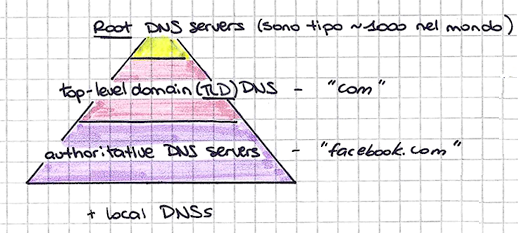
\includegraphics[width=1\linewidth]{Figures/02/dns-hiera.png}
  \end{center}
  \label{fig:gerarchia}
  \caption{Gerarchia a tre livelli dei DNS.}
\end{wrapfigure}

\noindent Si tratta di un database distribuito e di un protocollo a livello applicazione per inviare queries ai Server DNS, si occupa di \underline{tradurre} gli hostname\index{hostname} (e.g.: \textit{www.facebook.com}) nei corrispondenti indirizzi IP (e.g.: \textit{69.63.176.13}).\\

\noindent DNS offre servizi quali Host aliasing\index{host!aliasing} (tradurre un hostname in un altro hostname, spesso meno user-friendly di quello ricevuto), mail server aliasing, load distribution.\\

\noindent DNS Caching: stesso meccanismo del Web caching, ma applicato al DNS.\\

\noindent Resource Records (RR): informazioni immagazzinate nei database DNS. Sono triple della forma
\begin{verbatim}
    (Name, Value, Type, TTL)
\end{verbatim}
\noindent Dove TTL sta per Time-To-Live, tempo di vita del record nel database (scaduto il quale questo viene eliminato).

\begin{table}[h]
\begin{tabular}{|c|c|c|}
\hline
\textbf{Type} & \textbf{Name} & \textbf{Value}                                                \\ \hline
A             & hostname      & IP Address                                                    \\ \hline
NS           & domain        & hostname del DNS che sa ottenere l'IP degli host nel dominio  \\ \hline
CNAME         & host          & valore canonico per l'host che ha sinonimo *nome*             \\ \hline
MX            & host          & valore canonico di un mail server per host sinonimo di *nome* \\ \hline
\end{tabular}
\label{tab:rr}
\caption{Alcuni esempi di Resource Record. I valori dei campi ``Name'' e ``Value'' dipendono dal valore in ``Type''.}
\end{table}\index{resource record}

\addcontentsline{toc}{section}{Telnet}
\section*{\textcolor{RubineRed}{Telnet}}
\index{telnet}
\noindent Uno dei primi protocolli in assoluto per TCP/IP, basato su architettura client-server, molto semplice ma nella sua semplicità è deprecato, ora al suo posto si usa SSH (Secure SHell)\index{SSH}. Fondamentalmente Telnet permette di fare collegamenti ad altri terminali attraverso la rete (alla porta 23).\\

\noindent Come funziona: il client manda richieste al server Telnet, e quello risponde. Ogni tasto che viene battuto sulla tastiera del lato client, ogni singolo carattere, viene spedito sulla rete e ricevuto dal server. Il server, ricevuto un carattere, lo rimanda in risposta come una ``echo''. Quindi non stiamo parlando di digitare una parola o una frase e poi premere ``invio'' per inviarla al server, l'invio avviene lettera per lettera.\\Serve a fare accesso remoto ad altre macchine. Perché non si usa più e piuttosto si usa SSH? Perché Telnet trasmette in cleartext, ovvero: ogni carattere viene trasmesso in chiaro, senza essere cifrato in nessuna maniera. Attraversa la rete esattamente come viene scritto. Chiunque riesca a posizionarsi tra client e server potrebbe origliare ciò che viene detto e impossessarsi delle informazioni.

\addcontentsline{toc}{section}{Macchine Virtuali}
\section*{\textcolor{RedViolet}{Virtual Machines}}
\index{macchina virtuale}
\noindent (cenni).\\

\noindent Una Macchina Virtuale (VM), essenzialmente, è un software che, montato e avviato, è in grado di simulare un computer a sé stante istanziato all'interno del nostro computer. Virtualmente, è come se ritagliassimo qualche pezzetto hardware dal nostro computer e usassimo questi pezzetti per creare un computerino fatto dai ritagli del nostro computer. Ok, questo, ma a livello software. Senza segare letteralmente la CPU a metà.\\

\noindent Per fare ciò, presa un'immagine di un sistema operativo, dovremo usare un Hypervisor\index{hypervisor}, cioè un programma che virtualizza degli host usando l'hardware della nostra macchina. Se avete abbastanza risorse hardware, potreste anche avviare più di una macchina virtuale contemporaneamente! L'hypervisor che ci è stato consigliato si chiama \textbf{VirtualBox}\index{VirtualBox} di Oracle\footnote{https://www.virtualbox.org/wiki/Downloads}, in alternativa ce ne sono altre come VMWare Workstation\index{VMWare Workstation}. Perlomeno nelle versioni base, entrambi quelli che ho menzionato sono gratuiti.

\addcontentsline{toc}{section}{FTP}
\section*{\textcolor{Sepia}{FTP}}
\index{FTP}
\noindent \textcolor{Sepia}{F}ile \textcolor{Sepia}{T}ransfer \textcolor{Sepia}{P}rotocol. Protocollo per il trasferimento di files.\\

\begin{itemize}
    \item di tipo client-server;
    \item usa connessioni TCP su porte 20 e 21, entrambe aperte dal client:
    \begin{itemize}
        \item porta 20 per i dati;
        \item porta 21 per i comandi (controllo);
    \end{itemize}
    \item permette operazioni di upload e download;
    \item spesso oggi anziché usare FTP si preferisce scambiarsi file usando HTTP, perché come Telnet, anche in FTP tutte le informazioni transitano in chiaro, in formato ASCII.
\end{itemize}

\noindent Qualche comando FTP:
\begin{itemize}
    \item USER: username;
    \item PASS: password;
    \item LIST: elenca i contenuti della cartella;
    \item RETR: retrieve, richiedi un file;
    \item STORE: carica un file.
\end{itemize}

\noindent Come HTTP, FTP ha dei codici di stato (tipo il ``404 Not Found''). Alcuni codici sono:

\begin{itemize}
    \item 331 : username ok, password required;
    \item 125 : data connection already open; transfer starting;
    \item 425 : can't open data connection;
    \item 452 : error writing file;
\end{itemize}

\noindent Nel 99\% dei casi, FTP si usa da interfaccia a linea di comando (CLI): per avviare una connessione ftp, si usa il comando (è possibile autenticarsi anche come \texttt{anonymous})
\begin{verbatim}
    ftp <indirizzo>
\end{verbatim}

\noindent La questione PASV/PORT che forse vi interessa: in Windows 10, usare FTP può dare problemi a causa della questione della \textit{``modalità passiva/modalità port'' (PASV/PORT)}. PASV e PORT sono entrambi comandi per la connessione dati (una delle due porte usate da FTP, no? Dati e comandi, ecco, quella dei dati); la connessione dati FTP, a volte, viene ostacolata dai Firewall, quindi se in principio bastava usare il comando PORT, successivamente all'avvento di NAT e Firewall si è reso necessario aggiungere PASV, che non è altro che una modalità trasferimento dati compatibile con Firewall.

\addcontentsline{toc}{subsection}{tFTP}
\subsection*{\textcolor{Maroon}{tFTP}}
\index{tFTP}
\noindent Ovvero, \textcolor{Maroon}{t}rivial \textcolor{Maroon}{FTP}. A differenza di FTP, tFTP:
\begin{itemize}
    \item usa UDP (alla porta 69);
    \item ha pochissime funzioni (da cui il termine \textit{``trivial'', banale});
    \item non conosce il concetto di Directory (cartella);
    \item non usa autenticazione;
    \item ha quindi un utilizzo molto limitato;
    \item ha 2 modalità di trasferimento: ASCII (NETASCII) e binario (OCTET);
\end{itemize}

\noindent alcuni comandi tFTP:

\begin{itemize}
    \item \textbf{RR}: read request;
    \item \textbf{WR}: write request;
    \item \textbf{DATA}: dati;
    \item \textbf{ACK}: acknowledged;
    \item \textbf{ERR}: errore;
\end{itemize}

\noindent I pacchetti UDP inviati da tFTP sono a lunghezza fissa $= 512$ Bytes. La trasmissione si considera conclusa quando viene ricevuto un pacchetto di dimensioni $< 512$ B.

\addcontentsline{toc}{section}{SNMP}
\section*{\textcolor{WildStrawberry}{SNMP}}
\index{SNMP}
\noindent \textcolor{WildStrawberry}{S}imple \textcolor{WildStrawberry}{N}etwork \textcolor{WildStrawberry}{M}anagement \textcolor{WildStrawberry}{P}rotocol\\

\noindent Normalmente, se presente, la porta standard usata è 161 (UDP). Anche SNMP viene spesso bloccato dal firewall - com'è giusto che sia, visto che per design questo protocollo dovrebbe arrivare soltanto dall'interno.\\

\noindent Usato per gestione di reti, monitoraggio e configurazione di dispositivi di rete.\\

\noindent Consiste in un protocollo molto semplice che fa:
\begin{verbatim}
    GET - GETNEXT - GETBULK - SET - TRAP
\end{verbatim}

\noindent Fa uso di Access Control List (ACL)\index{access control list}, regole che indicano cosa può e cosa non può fare un dispositivo);\\

\noindent Si possono istanziare manager o agent ($\approx$ server, cioè un'entità che ha il suo database di MIB, Management Info Base) - ogni oggetto MIB è identificato da una serie di numeri in un formato tipo:
\begin{verbatim}
    1.3.6.1.2.1.1.3 = SysUptime
\end{verbatim}

\noindent E' un modo macchinoso di immagazzinare informazioni riguardo il device e la rete. Tutti quei numeretti sono come un sistema di coordinate GPS, l'interno di questi record somiglia vagamente a un JSON.
\newpage
\newpage
\addcontentsline{toc}{chapter}{DHCP}
\chapter*{\begin{center}DHCP\end{center}}
\hrulefill (argomento interno all'app layer)\hrulefill\\
\noindent \underline{D}ynamic \underline{H}ost \underline{C}onfiguration \underline{P}rotocol\index{DHCP} - serve a configurare gli host.\\
\noindent Problemi sorti nella decisione di \openapex come deve essere fatto un sistema di idnirizzamento:\begin{itemize}
    \item duplicazione degli indirizzi IP: che facciamo se qualcuno si assegna un indirizzo IP che già appartiene ad un altro Host?\footnote{Tra l'altro, e mi permetto di aggiungere ``ovviamente'', gli indirizzi IPv4. Per ovviare a questo problema, spesso si ricorre al NAT, Network Address Translation, che si fa anche per risparmiare sull'uso degli indirizzi IP pubblici.}
    \item riassegnazione degli indirizzi IP: ad esempio, come riassegniamo gli indirizzi quando spostiamo un ufficio da una sede ad una nuova sede fisica?
    \item spreco di indirizzi IP inutilizzati;
    \item interfaccia che renda possibile vedere tutti questi indirizzi;\footnote{se avete curiosità, fate un salto al sito \href{https://www.showmyip.com/}{showmyip.com/}}
\end{itemize}

\noindent Usando TCP, si possono usare 2 protocolli che si occupano di configurazione host (assegnano indirizzi IP in maniera automatica):
\begin{itemize}
    \item BOOTP\index{BOOTP} : funziona con i thin client (host senza disco), usa UDP;
    \item DHCP : come BOOTP, ma ulteriormente sviluppato. Introduce il parametro di \openapex lease'' : parametro di tempo, durante il quale l'host può usare l'indirizzo IP che DHCP gli ha assegnato (tipo un token di noleggio).
\end{itemize}

\noindent DHCP configura:
\begin{itemize}
    \item indirizzo IP;
    \item maschera di sottorete;
    \item indirizzi Gateway e DNS (ma non sempre);
    \item altri parametri.
\end{itemize}

\noindent L'addressing può avvenire in 3 modalità:
\begin{itemize}
    \item assegnazione manuale (o reservation): legata all'indirizzo MAC;
    \item assegnazione automatica: il tempo di lease normalmente è $=\infty$;
    \item assegnazione dinamica: il tempo di lease è molto breve $\approx 1h$;
\end{itemize}

\noindent L'addressing avviene in 4(+1) fasi:
\begin{enumerate}
    \item discover;
    \item offer;
    \item request;
    \item ack;
    \item release (non uso più l'indirizzo, i.e. ho spento il PC)*;
\end{enumerate}
\noindent \textcolor{Blue}{*È buona pratica che non si interrompa la connessione scollegando il cavo o mettendo il PC in standby quando si lascia un qualche luogo: così facendo, il DHCP non riesce a venire a sapere che la connessione è stata interrotta (si spreca l'indirizzo).}\\

\noindent \index{NETBEUI}\index{NETBIOS}\index{SAMBA}\textcolor{Blue}{Note di Lab: Il protocollo NETBEUI o NETBIOS (di Microsoft, nei sistemi Linux esiste il protocollo SAMBA), un vecchio protocollo di rete che funziona solo in locale. Il DNS di NETBEUI si chiama WINS (Windows Internet Name Service).}\\

\noindent Banalmente, per essere raggiungibile, il DHCP Server deve essere configurato con indirizzo Statico!\\

\noindent \index{DHCP!relay}DHCP Relay: funzione implementata nei router per cui le richieste DHCP dagli host vengono inoltrate ad un DHCP Server limitrofo. Se non c'è un DHCP Server a disposizione, un sistema Windows ha IP $169.254.0.0/16$.

\newpage
\addcontentsline{toc}{chapter}{Transport Layer}
\chapter*{\begin{center}Transport Layer\end{center}}
\begin{center}(Layer 4 nello stack TCP/IP)\end{center}\hrulefill \\
\noindent A livello di trasport, Internet utilizza due protocolli\footnote{nota: sebbene TCP e UDP siano i due protocolli più diffuso per il transport layer, non sono gli unici due protocolli esistenti per il trasporto in assoluto!}
\begin{itemize}
    \item TCP;
    \item UDP;
\end{itemize}
\noindent Sappiamo già che TCP è connection-oriented, con meccanismi di controllo della congestione e di flusso e di sicurezza etc., laddove invece UDP si limita a spedire il pacchetto dove gli viene indicato e Dio provvede di quello che succede al pacchetto.\\

\noindent Un pacchetto dati a livello di trasporto prende il nome di \underline{segmento:}\index{segmento} in alcuni documenti e RFC\footnote{non li avevo menzionati finora? RFC sta per Request For Comment, sono documenti che stabiliscono praticamente degli standard di questo e quel protocollo o meccanismo, li pubblicano svariati enti come la IETF.}, i segmenti vengono chiamati anche \openapex datagram'', ma con quel termine c'è un piccolo problema di ambiguità: infatti, con il termine \openapex datagram'' ci si riferisce anche ai pacchetti dati che raggiungono il livello di rete. Tutte le mie source utilizzano il termine \openapex segmento'', quindi magari usiamo quello e basta.\\

\noindent In genere, un segmento a livello di trasporto contiene tre elementi:
\begin{enumerate}
    \item nr. porta di origine / nr. porta di destinazione (campi lunghi 16 bits ciascuno, per un totale di $16+16=32$);
    \item altri campi di intestazione\footnote{useremo i termini \openapex intestazione'' e \openapex header'' intercambiabilmente.} (tipo e lunghezza variano tra TCP e UDP); 
    \item messaggio (il contenuto).
\end{enumerate}

\begin{figure} [h]
    \centering
    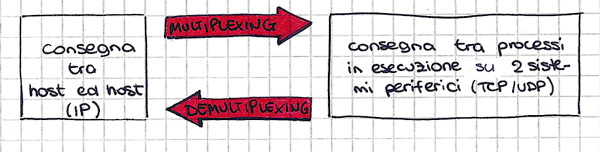
\includegraphics[width=0.75\linewidth]{Figures/03/mpx-dmpx.png}
\end{figure}


\noindent Multiplexing\index{multiplexing} a livello di trasporto: raduna diversi dati da diverse socket e li incapsula in un unico pacco di dati da spedire in rete (è importante che ogni socket abbia un numero di porta per completare questa operazione in avanti e indietro). In genere multiplexing è una qualche operazione che prende n input ed ha 1 output;\\

\noindent Demultiplexing\index{demultiplexing} a livello di trasporto: esamina determinati campi del messaggio ricevuto e decide a quale socket del ricevente consegnarlo. Qui stiamo parlando di ricevere da un unico input e di distribuire il contenuto ricevuto a n possibili output;\\

\noindent Sia TCP che UDP fanno MPXing e DMPXing.\\

\noindent \textit{Nota abbastanza importante sui numeri di porta\index{porta!numeri di}\index{porte!note}\index{porte!effimere}\index{porte!private}:
\begin{itemize}
    \item le porte numerate da $0\div1023$ vengono dette \openapex porte note'' perché sono riservate a servizi quali HTTP. Non si possono usare arbitrariamente per altre cose;
    \item le porte comprese tra $1024\div49552$ si chiamano \openapex indirizzi effimeri'', assegnati randomicamente al momento dell'apertura della porta;
    \item le porte comprese tra $49553\div65535$ sono \openapex porte private''.
\end{itemize}}
%%%%%%%%%%%%%%%%%%%%%%%%%%%%%%%%%%%%%%%%%%%%%%%%%%%%%%%%%%%%%%%%%
\addcontentsline{toc}{section}{UDP}
\section*{UDP}
\underline{U}ser \underline{D}atagram \underline{P}rotocol\index{UDP}
\begin{itemize}
    \item Protocollo connectionless - niente handshake a inizio connessione. Questo riduce notevolmente la congestione e rende così UDP per certi versi più veloce di TCP;
    \item \openapex senza fronzoli'': l'intestazione di un pacchetto UDP è lunga solo 8 Byte (contro quella di TCP che è lunga ben 20)
\end{itemize}

\noindent Header (intestazione) segmento UDP:
\index{UDP!header}
\begin{table}[h]
\begin{tabular}{cc}
\textit{(2 Bytes)}                                                               & \textit{(2 Bytes)}                                                                       \\ \hline
\multicolumn{1}{|c|}{\begin{tabular}[c]{@{}c@{}}Porta di\\ origine\end{tabular}} & \multicolumn{1}{c|}{\begin{tabular}[c]{@{}c@{}}Porta di\\ destinazione$^1$\end{tabular}} \\ \hline
\multicolumn{1}{|c|}{Lunghezza msg$^2$}                                          & \multicolumn{1}{c|}{checksum$^3$}                                                        \\ \hline
\end{tabular}
\end{table}
\noindent $^1$: usata per Demultiplexing;\\
$^2$: indica dove finisce il messaggio;\\
$^3$: per verificare errori nel messaggio: se i complementi a 1 sono andati a buon fine (e quindi anche l'invio/ricezione del pacchetto), il risultato del checksum deve essere uguale a $11111111$ $11111111$ (16 volte 1).\\
\index{checksum}
\noindent UDP non fa niente che non sia Multiplexing e Demultiplexing. Per la maggior parte dei protocolli dell'application layer (tipo HTTP) viene utilizzato TCP, perché TCP fornisce molti servizi legati alla stabilità e affidabilità della connessione. UDP viene usato perlopiù dove è richiesta non tanto correttezza di tutti i pacchetti ma piuttosto una alta responsiveness (quindi tempi d'attesa brevissimi) e ci si può permettere una certa percentuale di packet loss senza influire sul risultato visibile in maniera critica - quindi in servizi come streaming video o VoIP (voice over IP, ossia Skype, Discord etc., ma viste le performance di internet si sta iniziando ad usare TCP anche per questi qui).\\


\addcontentsline{toc}{section}{RTD}
\section*{RDT - Principi di Trasferimento Dati Affidabile}
\index{RDT}
\noindent Piccola digressione in cui parleremo, in maniera un po' teorica, del sistema di trasferimento dati affidabile (\underline{R}eliable \underline{D}ata \underline{T}ransfer, RDT): una serie di meccanismi da adottare per prevenire la perdita di informazione a seconda dei vari problemi che ci possono essere (ritardi, timeout, errori etc.). Questo perché TCP, per quanto premuroso possa essere come protocollo, si appoggia a protocolli a livello sottostante che non sono in grado di garantire davvero una comunicazione perfetta: qualcosa può andare male, e servono strategie per mitigare questo \openapex male''.
\addcontentsline{toc}{subsection}{RDT 1.0}
\subsection*{RDT 1.0 - Canale Affidabile}
\index{RDT!1.0}
\noindent L'approccio naïve, ovvero quello basato sull'assunzione che il canale sottostante sia perfettamente affidabile. Quindi non fa nulla di contromisure. 

\begin{figure} [ht]
    \centering
    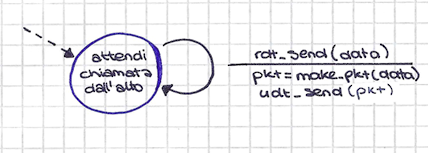
\includegraphics[width=0.8\linewidth]{Figures/03/rdt1-0-mit.png}
    \caption{RDT 1.0, lato mittente. Spieghino veloce di cosa succede qui: c'è uno stato solo, in cui il mittente attende la chiamata dall'alto (ovvero dal layer sopra); quando riceve il comando \openapex send(data)'', risponde con 2 azioni - crea il pacchetto con i dati e le info necessarie, e lo invia.}
\end{figure}

\begin{figure} [h!]
    \centering
    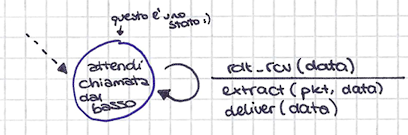
\includegraphics[width=0.8\linewidth]{Figures/03/rdt1-0-rcv.png}
    \caption{RDT 1.0, lato ricevente. Quando viene ricevuta una chiamata \openapex receive(data)'', estrae i dati dal pacchetto (extract) e li consegna al layer sopra (deliver). Come dicevamo, nessuno dei due lati fa nient'altro.}
\end{figure}
\newpage

\addcontentsline{toc}{subsection}{RDT 2.0}
\subsection*{RDT 2.0 - Rilevamento Errori}
\index{RDT!2.0}
\noindent Supponiamo ora che ci possano essere errori. Dobbiamo quindi fare in modo che il lato ricevente dia un feedback (ACK, NAK). Chiamiamo questo approccio error detection-feedback-retransmission.\footnote{La famiglia di protocolli che fanno questo tipo di cosa si chiama ARQ, Automatic Repeat reQuest (o Query).}

\begin{figure} [h]
    \centering
    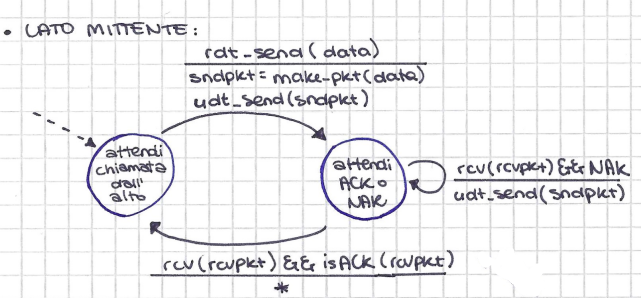
\includegraphics[width=0.75\linewidth]{Figures/03/rdt2-0-snd.png}
    \caption{RDT 2.0, lato mittente. Questo ha 2 stati, uno di attesa chiamata e uno di attesa feedback: RDT riceve la chiamata \openapex send'', quindi impacchetta, spedisce il messaggio e si mette in attesa di feedback. Se arriva un NAK (ovvero errore rilevato), allora rispedisce lo stesso pacchetto di nuovo; altrimenti (ACK), torna in attesa che il layer sopra gli passi un nuovo pacchetto da inviare.}
    \label{fig:rdt2.0s}
\end{figure}

\begin{figure} [h]
    \centering
    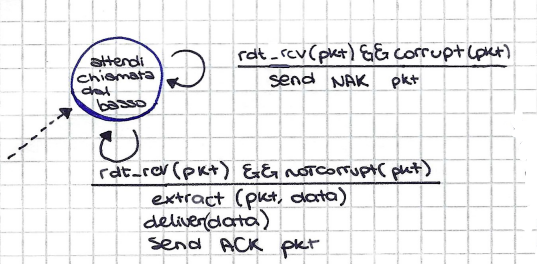
\includegraphics[width=0.6\linewidth]{Figures/03/rdt2-0-rcv.png}
    \caption{RDT 2.0, lato ricevente. Qui, all'arrivo di un messaggio dal layer sottostante, possono succedere 2 cose: il pacchetto non va bene (corrupt) $\rightarrow$ invia NAK in risposta; il pacchetto va bene $\rightarrow$ risponde ACK al mittente e consegna il pacchetto al layer sopra.}
    \label{fig:rdt2.0r}
\end{figure}
\newpage
\noindent Semplice semplice. Ora però sorge un altro problema ancora: e se fosse il pacchetto contenente \openapex ACK/NAK'' ad essere corrotto? $\rightarrow$ soluzione: aggiungere ad ogni pacchetto un nuovo campo di informazione: il Sequence Number\index{sequence number}. Tipicamente vengono usati numeri naturali crescenti, ma è sufficiente anche alternare messaggi con SN 0 e SN 1 perché la magia funzioni.


\bigskip
\addcontentsline{toc}{subsection}{RDT 2.1}
\subsection*{RDT 2.1 - Sequence Numbers}
\index{RDT!2.1}
\begin{figure} [h]
    \centering
    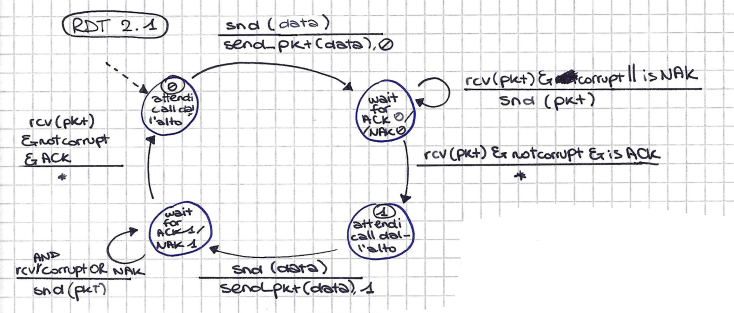
\includegraphics[width=0.7\linewidth]{Figures/03/rdt2-1-s.png}
    \caption{RDT 2.1, lato mittente: questo qui fondamentalmente dice: se il pacchetto di feedback arriva corrotto o contentente un NAK, in base allo stato dell'automa in cui mi trovo o rispedisco il pacchetto con SN = 0 oppure quello con SN = 1; in questa maniera, se il destinatario aveva capito il messaggio con SN 0 e il mittente gli manda un pacchetto con lo stesso SN, il destinatario si rende conto che è una ripetizione e non una nuova trasmissione. (E questo credo sia tutto ciò che cambia lato destinatario, spero sia la ragione per cui ho omesso l'automa del lato destinatario interamente)}
    \label{fig:rdt-21s}
\end{figure}

\newpage
\addcontentsline{toc}{subsection}{RDT 2.2 e RDT 3.0}
\subsection*{RDT 2.2 e 3.0 - ACK duplicati e Time-out}
\index{RDT!2.2}\index{RDT!3.0}\index{ACK!duplicati}\index{time-out}
\noindent In breve, RDT 2.2 introduce al posto di ACK e NAK, soltanto l'uso di ACK ma duplicati, nel senso: invece di mandare un messaggio del tipo \openapex non ho capito questo'' dice \openapex l'ultimo messaggio che ho capito bene è quello'' (identificando \textit{questo e quello} con i sequence number dei messaggi in questione.);\\
\noindent RDT 3.0 introduce il meccanismo di Time-out: è possibile che un pacchetto si smarrisca per strada, quindi si fa uso di una sorta di countdown per ogni pacchetto - un timer, se vogliamo - per stabilire se e quando smettere di aspettare un riscontro.\\
\noindent Credo e spero che non valga la pena annettere gli automi che illustrano il funzionamento anche di questi due, perché sono sempre più densi di stati e comportamento che trovo più facile riassumere a parole. È una scelta che invecchierà male? Lo scopriremo (ma non credo).\\

\noindent E questi sono protocolli di tipo \openapex Stop-and-Wait''\index{protocollo!stop-and-wait} che approcciano il problema della gestione degli errori tramite attesa di feedback o time-out; ora vedremo il GO-BACK-N, che è una famiglia di protocolli che ha a che fare con il \openapex pipelining''\index{pipelining} - ovvero, invece di fermarsi ad aspettare feedback ogni volta che si manda un singolo pacchetto, se ne mandano $n$ uno dietro l'altro. È indubbiamente più efficiente, ma quanti pacchetti posso mandare in sicurezza senza che un errore a un certo punto generi fatalmente \textit{chaos \& confusion}?

\addcontentsline{toc}{subsection}{Go-Back-N}
\subsection*{Go-Back-N}
\index{Go-Back-N}
\noindent Per rispondere alla domanda di cui sopra, si fa uso di quella che viene chiamata \index{finestra scorrevole}\openapex finestra scorrevole''\footnote{da non confondere con la finestra di congestione, meccanismo di controllo congestione TCP (TCP Reno).}: la larghezza di questa finestra cambia dinamicamente ma non a caso, la dimensione della finestra viene adattata dal controllo di flow e congestione!\index{congestione}

\begin{figure} [h]
    \centering
    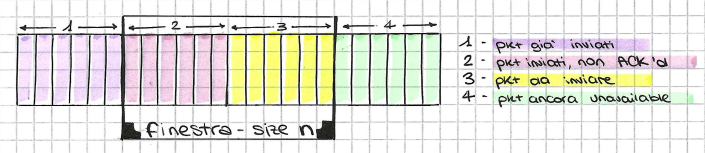
\includegraphics[width=1\linewidth]{Figures//03/window.png}
    \caption{Quanto mi piace usare 'sti colori. Finestra scorrevole, con annessa adorabile legenda dei colori. L'ultima parola a destra nel punto 4 è \openapex unavailable'', ndr.}
    \label{fig:congwin}
\end{figure}

\noindent Riscontro cumulativo\index{riscontro cumulativo}: mandare un ACK per il pacchetto numero N implica che tutti i messaggi fino ad N sono stati ricevuti correttamente $\approx$ \openapex fino a N li ho capiti tutti''. In caso di time-out, il mittente rispedisce tutti i pacchetti della zona 2 (in rosa\footnote{pastello! :D}), cioè quelli inviati ma non confermati da ACK.\\
\noindent Selective Repeat (SR)\index{selective repeat}: \openapex non ritrasmettere tutto quanto, ma solo le parti che non ho capito'' (starà poi al ricevente metterli nel giusto ordine quando vengono ritrasmessi e ricevuti).

\addcontentsline{toc}{section}{TCP}
\section*{TCP}
\index{TCP}
\underline{T}ransmission \underline{C}ontrol \underline{P}rotocol\\

\epigraph{With TCP, two hosts are a company, and three are a crowd.}{\textit{Una qualche edizione del Kurose-Ross}}

\begin{itemize}
    \item connection-oriented: prevede che si faccia un handshake (lit. \openapex stretta di mano'') prima di iniziare lo scambio di messaggi vero e proprio;
    \item sempre point-to-point: connette un solo host con un solo host, fine.
\end{itemize}

\noindent Fantastici parametri TCP e a quali sigle trovarli:
\index{TCP!parametri}
\begin{itemize}
    \item \index{MSS}MSS, Maximum Segment Size: limite di dati che possono essere messi in un segmento TCP. Questo parametro dipende dal (vedi punto successivo)
    \item \index{MTU}MTU, Maximum Transmission Unit: dimensione massima dei dati che possono essere gestiti al livello datalink - ad esempio, Ethernet ha una MTU di 1500 Bytes;
    \item \index{TCP!flag}Flag TCP! Da ricordare. Sono bit (quindi valori di lunghezza 1 che possono essere o $=0$ o $=1$). Vediamole:
    \begin{itemize}
        \item RST: sta per \openapex ReSeT'', si usa in caso di gravi errori;
        \item PSH: (PUSH, credo) indica al ricevente di passare subito questo segmento al layer soprastante, senza elaborare niente;
        \item URG: manca il contenuto del segmento come URGente;
        \item FIN e SYN: si usano rispettivamente per indicare una chiusura e un'apertura della connessione; 
        \item ISN: Initial Sequence Number: numero generato in modo pseudorandomico all'avvio di una connessione TCP. È compreso tra i valori $0\div(2^{32}-1)$, da quel numero in poi si conteranno i sequence number (tipicamente in modo crescente, andando di successori);
        \item MSL: Max Segment Lifetime, il tempo durante il cui il segmento resterà in vita nella rete. Scaduto questo tempo, il pacchetto viene soppresso;
        \item CWR e ECE, le vedremo più avanti.
    \end{itemize}
    Queste flag appaiono nel header TCP nel seguente ordine: CWR - ECE - URG - ACK - PSH - RST - SYN - FIN;
\end{itemize}

\noindent Fattore di Time-out: ci interessa che il Time-out sia maggiore del RTT (round-trip time), naturalmente, altrimenti il pacchetto non ha nemmeno modo di arrivare a destinazione perché muore prima. In TCP, il RTT viene preso ad ogni ACK. Non può essere stabilito a priori, al limite si può stimare.\\

\noindent estimatedRTT:
\[eRTT = (1-\alpha)\cdot eRTT + \alpha \cdot sampleRTT\]
\noindent $\alpha$ è un fattore costante, di solito $=0,125$, per fare una media pesata di quei due parametri; $sampleRTT$ è il RTT misurato \textit{(sampled)} per ogni andata e ritorno.\\

\[devRTT = (1-\beta)\cdot devRTT + \beta \cdot (sampleRTT - eRTT)\]
\noindent con $\beta = 0,25$, questa è la deviazione standard RTT. Alla fine, il RTT calcolato avrà valori che convergono in modo abbastanza stabile, e la deviazione standard valori abbastanza bassi.\\

\noindent Notine di dubbia utilità di lab:
\begin{itemize}
    \item TSHARK non è altro che Wireshark ma con una interfaccia command line anziché interfaccia grafica;
    \item Wireshark ha un tool per l'analisi RTT: \begin{verbatim}
        tcp.analysis.ack_rtt
    \end{verbatim}
\end{itemize}

\noindent \index{RTO}RTO: Retransmission Time-Out: tempo entro cui la sorgente si aspetta di ricevere un riscontro. Non può essere un valore statico predefinito, dipende da moltissimi fattori. Si calcola dinamicamente (perché basato sul RTT, che si calcola dinamicamente), di solito il risultato è compreso tra $200ms<RTO<60+sec$:
\[RTO = eRTT + 4 \cdot devRTT\]

\noindent \index{window!receive}RcvWindow: Buffer che serve ad evitare problemi di flusso dei dati. Memorizza i byte ricevuti per poi passarli all'app layer. Quando questo buffer è pieno, il destinatario manda byte di controllo al sender per dire che non può ricevere nient'altro al momento. Appena si liberano $n$ bytes, il destinatario\footnote{probabilmente per abitudine tenderò ad abbreviare mittente e destinatario con snd e rcv qualche volta (sender, receiver), sapevatelo} invia un messaggio al mittente per dire \openapex Ok, ora ho spazio, mi aspetto messaggi a partire da $<$(ultimo messaggio ricevuto $+1>$ e ho $n$ byte di spazio.''
\newpage
\addcontentsline{toc}{subsection}{Handshake TCP}
\subsection*{\textcolor{blue}{SYN-SYNACK-ACK, il Three-Way Handshake in TCP}}
\noindent \index{handshake!three-way}\index{TCP!handshake}È un concetto abbastanza importante. Fondamentalmente questo è ciò che va fatto prima di avviare ogni conversazione tra host TCP. È come quando al telefono ci si risponde \openapex Pronto, chi è?'' \openapex Sono Tizio, tu sei Caio?'' \openapex Ciao Tizio, sì io sono Caio''. Una fase di autenticazione preliminare, insomma. Fatto questo, si può iniziare la conversazione vera e propria.\\

\begin{figure} [h]
    \centering
    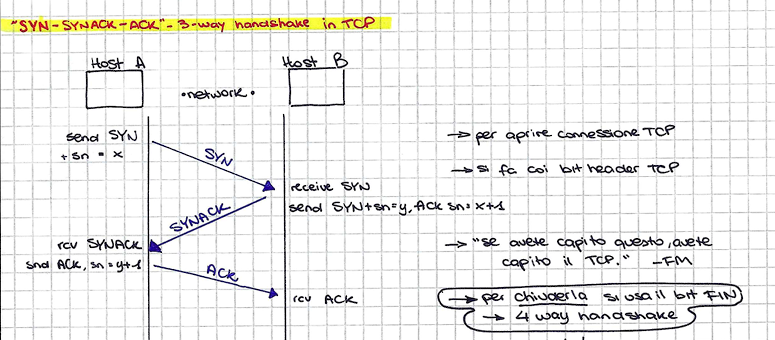
\includegraphics[width=1\linewidth]{Figures/03/tcp-3whs.png}
    \caption{Three-way handshake TCP.}
    \label{fig:3whsTCP}
\end{figure}

\noindent Finita la conversazione, per continuare la metafora della telefonata, vogliamo segnalare che abbiamo finito di parlare, quindi dire una cosa come \noindent Va bene, ora ti saluto, ciao!'', a cui l'interlocutore risponde \noindent OK, ciao!'' e poi si riattacca. Paradossalmente questo si fa in 4 messaggi, più di quanti non ce ne vogliano per iniziare la conversazione - ma queste sono le meraviglie di TCP. Comunque, \index{handshake!four-way}4-way handshake di chiusura in Fig. \ref{fig:4whsTCP}:

\begin{figure} [h]
    \centering
    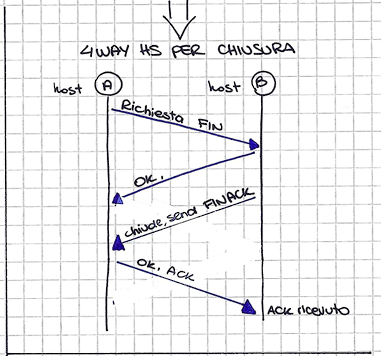
\includegraphics[width=0.5\linewidth]{Figures/03/4whstcp.png}
    \caption{Handshake di chiusura TCP.}
    \label{fig:4whsTCP}
\end{figure}

\noindent Controllo della congestione, nota: immettere in rete dei \openapex pacchetti di controllo'' a scopo di controllo della congestione è fortemente sconsigliato, paradossalmente congestiona esso stesso la rete.\\

\noindent Il discorso su prestazioni e scenari relativi è discusso in maniera molto esaustiva sia nel libro che nelle slides, you're on your own with this one $>:)$\\

\noindent Comunque ci sono due approcci principali al \index{controllo congestione}congestion control: End-to-End e Network-assisted. Per quanto riguarda TCP e il congestion control, occorre parlare di finestra di congestione\index{finestra di congestione}.\\
\noindent congWindow: finestra di congestione. Quantità di dati riscontrati da un host durante la connessione. Vincolo: TCP non può inviare dati ad un rate maggiore della ampiezza della finestra di congestione, e questa finestra, come ha senso che sia, cambia ampiezza dinamicamente a seconda del livello corrente di congestione. Per cambiare il ritmo di invio in funzione della congestione si usano diversi approcci (io qui li ho chiamati Algoritmi, non so se sia accurato come termine, ma penso stessi facendo riferimento ai TCP Tahoe e Reno)\index{TCP!Tahoe}\index{TCP!Reno}:
    \begin{itemize}
        \item AIMD: incremento additivo, decremento moltiplicativo;
        \item Slow Start: per ogni ACK ricevuto, raddoppio la dim. della finestra;
        \item Fast Recovery: questo non lo vedremo, rip
    \end{itemize}
\noindent Threshold (soglia): limite tra decremento moltiplicativo e incremento additivo: se il valore corrente è $<Thr \rightarrow$ si adotta slow start; se il valore corrente è $>Thr\rightarrow$ si adotta congestion avoidance (AIMD). Nel modulo di tutorato si vedono meglio questi discorsi con TCP Reno e compangia. Comunque, l'idea è che l'algoritmo vada a convergere e stabilizzarsi su un certo range di rata di trasmissione, anche se nella pratica poi non va così (vedasi TCP CUBIC, non ho nessuna memoria di cosa sia questa roba).\\

\addcontentsline{toc}{subsection}{Note di Lab}
\subsection*{\textcolor{RoyalPurple}{Note di Lab:}}
Nmap, network scanner! 2 tecniche principali:\index{nmap}
\begin{itemize}
    \item PORTSCAN\index{port!scanning}: attività promiscua (losca, sospetta), da usare solo previa autorizzazione se non vogliamo cacciarci in qualche guaio, perché il port scanning di solito è una tecnica utilizzata per scoprire porte aperte in altri dispositivi, al fine di sfruttarne le vulnerabilità e provare qualche attacco. Port scanning aiuta un malintenzionato a trovare porte aperte e a capire se queste sono in ascolto o stanno trasmettendo dati. Inoltre, può rivelare misure di sicurezza (come un firewall) sono in uso in qualche rete aziendale\footnote{ fonte \href{https://www.fortinet.com/resources/cyberglossary/what-is-port-scan}{Qui}};
    \item PING SWEEP\index{ping!sweep}: port monitoring, analisi di sicurezza, information gathering, attacchi, beh suona abbastanza simile al port scanning. Il ping sweeping consiste in mandare messaggi di ping a più indirizzi IP per trovare degli host \openapex vivi'' (insomma accesi) nella rete, da cui poi si procede col port scanning sugli host vivi.\footnote{Se volete divertirvi a leggere/guardare, ho trovato \href{https://study.com/academy/lesson/ping-sweeps-definition-tools-uses.html}{questo}}
\end{itemize}
\texttt{nmap} utilizza delle \openapex fingerprints'' (impronte digitali) per raccogliere informazioni su di un target. Eventualmente è possibile utilizzarlo con interfaccia grafica (che si chiama Zenmap), ma \textit{il prof, con un velo di sarcasmo, ci fa sapere che \openapex Zenmap è per quegli utenti che usano il Mac''.} Nmap ha incorporato uno script engine in LUA, ovvero una collezione di script che si possono eseguire per trovare vulnerabilità e affini. Basta eseguire il comando \begin{verbatim}
    nmap --script-updatedb
\end{verbatim}
per aggiornare questa fantastica lista di script curata dagli eroi invisibili della rete.\\
\noindent ncat invece è un tool open source a riga di comando utile a collegarsi ad un altro host da remoto, pretty cool. Tutte le info che abbiamo visto di ncat si trovano nelle slides del prof - a \href{https://computerscience.unicam.it/marcantoni/}{questo indirizzo}, nella tabella \openapex didattica'' $>$ Internet, Reti e Sicurezza $>$ Esercitazioni e Laboratorio Wireshark al nome \openapex nmap.pdf''.
\newpage
\addcontentsline{toc}{chapter}{Network Layer}
\chapter*{\begin{center}Network Layer\end{center}}
\begin{center}(Layer 3 nello stack TCP/IP)\end{center}
\hrulefill \\

\noindent Per iniziare, il Network Layer può essere diviso in due macro-componenti che interagiscono fra di loro: \index{plane!data}\index{plane!control}Data Plane e Control Plane (dove Plane significa piano, strato). A questo layer dello stack, la PDU si chiama Datagramma.\index{datagramma}\\

\noindent Nel Data Plane vengono trattate tutte le funzioni \openapex pre-router'', incluso il tradizionale IP Forwarding che vedremo a breve.\\

\noindent Forwarding VS Routing:\index{forwarding}\index{routing}
\begin{itemize}
    \item Forwarding: azione svolta dal router, consiste nel trasferire un pacchetto da una input link interface alla opportuna output link interface;
    \item Routing: azione svolta a livello di rete, comprende TUTTO il processo per determinare il percorso (path) che il pacchetto percorre da mittente al destinatario.
\end{itemize}
\noindent N.B.: i protocolli di routing $\neq$ protocolli routabili\index{protocollo!routabile} ($\approx$ instradabili\footnote{protocollo utilizzato per mandare dati attraverso più reti, selezionando i formati dati opportuni in base alle reti in questione. Tipo IP. IP non decide nulla a livello di percorsi attraverso la rete (non è un protocollo di routing, ma routabile).}). Also, in internet non esistono (e non possono esistere) due indirizzi uguali corrispondenti a due diversi Host.\\

\addcontentsline{toc}{section}{IP}
\section*{\textcolor{WildStrawberry}{IP}}
\index{IP}
\underline{I}nternet \underline{P}rotocol\\

\noindent Definisce il modo in cui i pacchetti sono instradati.\\
\addcontentsline{toc}{subsection}{Datagramma IPv4}
\subsection*{Datagramma IPv4}
\index{IPv4}
\index{IPv4!datagramma}

\begin{figure} [h]
    \centering
    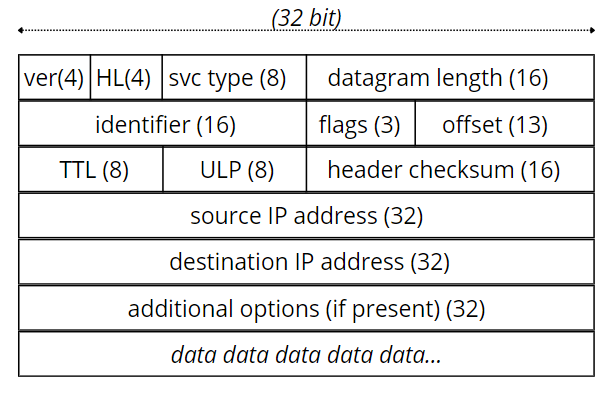
\includegraphics[width=0.5\linewidth]{Figures/04/headerIPv4.png}
    \caption{Struttura di un header IPv4. Tra parentesi sono indicati i bit di lunghezza di ciascun campo.}
    \label{fig:headipv4}

\end{figure}

\noindent In Figura \ref{fig:headipv4} è raffigurata la struttura di un header (intestazione) a livello di rete, nello specifico un header IP, versione 4 (esiste anche IPv6, lo vedremo brevemente più avanti). Le varie sigle stanno per:
\begin{itemize}
    \item ver: \textit{versione;}
    \item HL: \textit{header length}, lunghezza header;
    \item svc type: \textit{service type;}
    \item TTL: \textit{Time-To-Live;}
    \item ULP: \textit{Upper Layer Protocol,} ovvero che protocollo aspettarsi al layer immediatamente superiore (i.e., il layer di trasporto, quindi solitamente TCP o UDP);
\end{itemize}

\noindent N.B.: il time-to-live, sebbene esprima un concetto di \openapex tempo'', non è un valore da intendersi come un timer di ore e minuti, una cosa tipo \textit{hh:mm:ss}: è una unità di tempo \textit{logica}, ovvero un contatore a $n$ che viene decrementato di 1 ogni volta che un pacchetto arriva ad un router\footnote{Per capirci, invece di contare quanto tempo impiegate per arrivare dalla porta del bagno a quella della cucina, contate i passi che fate. I passi, coi piedi, i passi fisici.}. Se il TTL arriva a $=0$, allora il pacchetto viene dichiarato morto: questo per evitare che i pacchetti entrino per errore in circolo all'infinito tra i vari router della rete.\\

\noindent IPv6,\index{IPv6} come datagramma, è molto simile a IPv4 ma con qualche differenza, la più rilevante credo sia nelle dimensioni dell'indirizzo - non più 32 ma 128 bit - ed altre differenze nei contenuti.\footnote{Da qualche parte che non so dirvi al momento, esistono tools e metodi per convertire un indirizzo IPv4 in IPv6 e viceversa. Penso basti andarseli a cercare sul web.}\\

\noindent Interfaccia di rete\index{rete!interfaccia}: punto di connessione tra host e router (e.g.: una scheda Bluetooth, Ethernet, etc.). Ciascuna interfaccia di rete può avere più IP Address associati.\\

\addcontentsline{toc}{subsection}{Indirizzamenti}
\subsection*{Evoluzione degli Indirizzamenti}
\noindent Ovvero, piccolo excursus storico.\\

\begin{itemize}
    \item 1981 - Indirizzamento a 2 livelli \underline{classful}\index{indirizzi!classful}: semplice da comprendere e implementare, questo tipo di addressing architecture si basa sulla divisione in 5 classi di indirizzi, basate sui primi 4 bit dell'indirizzo IPv4. In questa architettura 2-layer classful, la struttura dell'indirizzo IP era: \begin{verbatim}
        (network_ID).(host_ID)
    \end{verbatim}
    la prima metà dell'indirizzo identificava la rete, la seconda metà l'host. Quindi la classe (identificata nei primi 4 bit a sinistra) è associata alla rete!

\begin{table}[h]
\centering
\begin{tabular}{cc}
classe                                                                                                         & \multicolumn{1}{l}{start address (decimale e binario)}                                            \\ \hline
\multicolumn{1}{|c|}{classe A}                                                                                 & \multicolumn{1}{c|}{\begin{tabular}[c]{@{}c@{}}0.0.0.0\\ \hl{0000}0000.00000000. (...)\end{tabular}}   \\ \hline
\multicolumn{1}{|c|}{classe B}                                                                                 & \multicolumn{1}{c|}{\begin{tabular}[c]{@{}c@{}}128.0.0.0\\ \hl{1000}000.00000000. (...)\end{tabular}}  \\ \hline
\multicolumn{1}{|c|}{classe C}                                                                                 & \multicolumn{1}{c|}{\begin{tabular}[c]{@{}c@{}}192.0.0.0\\ \hl{1100}0000.00000000. (...)\end{tabular}} \\ \hline
\multicolumn{1}{|c|}{\begin{tabular}[c]{@{}c@{}}classe D\\ \textit{(multicast)}\end{tabular}} & \multicolumn{1}{c|}{\begin{tabular}[c]{@{}c@{}}224.0.0.0\\ \hl{1110}0000.00000000. (...)\end{tabular}} \\ \hline
\multicolumn{1}{|c|}{\begin{tabular}[c]{@{}c@{}}classe E\\ \textit{(reserved)}\end{tabular}}  & \multicolumn{1}{c|}{\begin{tabular}[c]{@{}c@{}}240.0.0.0\\ \hl{1111}0000.00000000. (...)\end{tabular}} \\ \hline
\end{tabular}
\end{table}

    Questo sistema 2-layer classful è deprecato, non più in uso, ma talvolta viene chiesto all'esame, quindi il mio consiglio spassionato è: esercitatevi a convertire i numeri dal decimale al binario o memorizzate i numeri che delimitano le classi (0, 128, 192, 224 e 240. Gli intervalli, naturalmente, sono $0\div127$, $128\div191$, $192\div223$, $224\div239$ e $240\div255$.);
\item 1984 - Indirizzamento a 3 livelli classful: la struttura dell'indirizzo non è più: \begin{verbatim}
        (network_ID).(host_ID)
    \end{verbatim}
ma cambia in: \begin{verbatim}
        (network_ID).(subnet_ID).(host_ID)
    \end{verbatim}

Il subnetting è un argomento che vedremo tra un attimo;
\item 1993 - CIDR (Classless Inter-Domaining Routing)\index{CIDR}: viene eliminata la divisione in classi; indirizzi vengono gestiti in modo efficiente per fare routing a questa maniera \begin{verbatim}
    IP = < prefisso, suffisso >
\end{verbatim} 
dove il prefisso indica la rete e il suffisso indica l'host connesso alla rete. È una forma di subnetting\index{subnetting}, la dimensione di questi due campi varia arbitrariamente! Per risalire a dove inizia uno e dove finisce l'altro, per distinguerli tra di loro occorre usare un'altra stringa di bit chiamata \hl{maschera di rete} (netmask): la netmask\index{netmask}\index{rete!maschera} è una stringa di 32 bit disposti in una sequenza di $x$ bit \openapex 1'' seguiti da $y$ volte \openapex 0'' (ovviamente, $x+y$ deve tornare 32), tipo:
\begin{verbatim}
    11111111.11111111.11111111.00000000
\end{verbatim}
\noindent questo è il caso di una netmask $/24$ (cosiddetta \textit{barra 24,} ovvero, 24 bit `1' seguiti da 8 bit `0').
Facendo l'operazione di AND logico tra la netmask e l'indirizzo CIDR, possiamo separare la parte di rete dalla parte di host (rispettivamente nel prefisso e suffisso).
\end{itemize}

\noindent Indirizzi IP da ricordare (particolari, riservati a questo scopo unico):
\begin{itemize}
    \item $0.0.0.0$ : indirizzo di avvio stack TCP/IP;
    \item $127.0.0.1$ : indirizzo di loopback\index{indirizzo!loopback} a localhost\index{localhost}. Permette di comunicare con la propria stessa macchina come se fosse un altro host in rete (per fare una metafora personale, è come parlare alla propria immagine riflessa, il messaggio è indirizzato a me stess* e \textit{rimbalza} sulla superficie dello specchio tornando a me). Perché dovrei voler comunicare con me stesso? Boh, per fare test;
    \item $<net\_ID>$ seguito da tutti $1$ : indirizzo di Broadcast\index{indirizzo!broadcast}. Manda pacchetti a TUTTA la rete contrassegnata dall'indirizzo $<net\_ID>$;
    \item $<net\_ID>$ seguito da tutti $0$ : indirizzo\index{indirizzo!di rete} di rete (o sottorete), non identifica un host.
    \item $255.255.255.255$ (in binario, sono 32 volte $1$) : broadcast\index{indirizzo!broadcast locale} locale.
\end{itemize}
\newpage
\addcontentsline{toc}{subsection}{Subnetting}
\subsection*{Subnetting}
\index{subnetting}
\noindent Ovvero, dividere logicamente (non fisicamente) la rete in sotto-reti da TOT indirizzi ciascuna usando maschere di rete.

\begin{table}[h]
\centering
\begin{tabular}{|ll|l|}
\hline
\multicolumn{2}{|l|}{\textit{(prefisso di rete)}} &          \\ \hline
\multicolumn{1}{|c|}{net\_ID}     & subnet\_ID    & host\_ID \\ \hline
\end{tabular}
\end{table}

\noindent Quanto è lungo il prefisso di rete?\index{rete!prefisso} Dipende: in caso di subnetting\index{subnetting!statico} statico, ha lunghezza fissa; nel caso di subnetting dinamico\index{subnetting!dinamico} (Variable Length Subnet Mask, VLSM),\index{VLSM} ha lunghezza variabile.\footnote{Potete usare \href{https://subnettingpractice.com/vlsm.html}{questo tool online} per verificare la correttezza delle vostre subnet quando fate esercizi di subnetting :)}\\

\noindent Esempio: risaliamo alla rete, dato l'indirizzo\begin{verbatim}
    193.205.92.150/25
\end{verbatim}

\noindent Per risalire alla rete, facciamo un AND logico con la netmask a barra 25 (cioè con 25 volte 1 seguìti da 7 volte 0):
\begin{verbatim}
11000001.11001101.01011100.10010110
\end{verbatim}
$(\land)$
\begin{verbatim}
11111111.11111111.11111111.10000000 =
\end{verbatim}

\begin{verbatim}
11000001.11001101.01011100.10000000
\end{verbatim}
che, tradotto da binario a decimale, sarebbe\begin{verbatim}
    193.205.92.128
\end{verbatim}

\noindent Ci verrà anche richiesto il procedimento opposto, allo scopo di progettare reti e sottoreti: partendo da un indirizzo e una barra, determinare quante e quali sottoreti assegnare (e per ciascuna, quanti host si possono assegnare).\\

\noindent Alle volte è buona pratica assegnare la barra di sottorete un numero più alta del minimo indispensabile (cioè raddoppiare gli host disponibili, che è ciò che succede se si alloca un altro bit agli host): ad esempio se abbiamo 62 host già assegnati, è meglio non andare per una netmask a /24 (che offre 64 indirizzi, solo 2 in più di quelli che abbiamo già), altrimenti appena ne vogliamo aggiungere altri 3 quella sottorete non ci basterà più! E tocca riconfigurare tutto da capo. Quindi meglio una /23. Accontentatevi di una /24 solo nel caso in cui l'esercizio dice \openapex sappiamo già che non intendono apportare espansioni alla rete in futuro''.
\newpage
\addcontentsline{toc}{chapter}{Data Link e LAN}
\chapter*{\begin{center}\texttt{Datalink e LAN}\end{center}}
\hrulefill \\
\addcontentsline{toc}{section}{LAN}
\section*{\textcolor{RedViolet}{LAN}}
\noindent \underline{L}ocal \underline{A}rea \underline{N}etwork\\
\index{LAN}\index{data link}
\noindent LAN, Definizione del IEEE: Sistema di comunicazione che permette ad apparecchiature indipendenti di comunicare tra loro entro un'area delimitata, utilizzando un canale fisico ad elevata velocità e con basso tasso d'errore.\\

\begin{itemize}
    \item tipicamente, non sono trasmissioni di dati continue, ma a \openapex burst'', cioè a intervalli, a raffiche discontinue;
    \item tutte le macchine della LAN condividono lo stesso canale fisico di comunicazione;
    \item è una rete...
    \begin{itemize}
        \item economica;
        \item facile da modificare;
        \item di facile manutenzione;
        \item capace di sopportare grossi carichi di dati;
        \item duratura nel tempo (anni, se ben progettata e configurata).
    \end{itemize}
\end{itemize}
\noindent Aspetti meno piacevoli e delicati della LAN:
\begin{itemize}
    \item tutti gli host collegati devono essere identificati;
    \item bisogna stabilire delle regole per permettere agli host di comunicare tra di loro;
    \item flessibilità - compatibilità tra host di natura diversa (pensate ad un dispositivo mobile, un Desktop Computer, un sensore);
    \item modularità;
    \item espandibilità;
    \item gestibilità (vedere SNMP, protocollo Applicativo visto nel capitolo Application Layer);
\end{itemize}


\begin{wrapfigure}{r}{0.6\textwidth}
 \begin{center}
 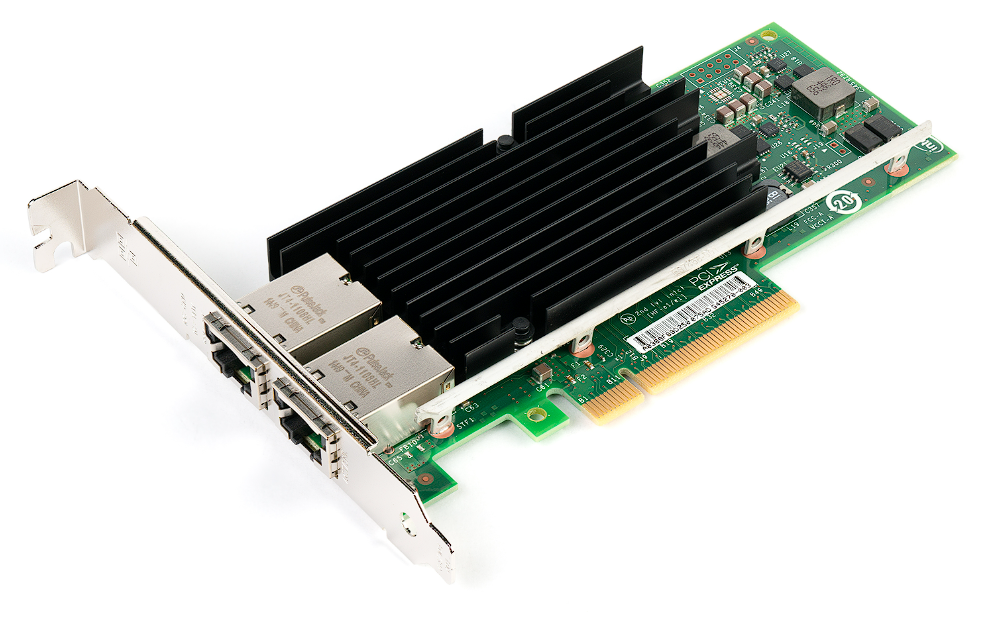
\includegraphics[width=1\linewidth]{Figures/05/nic.png}
  \end{center}
  \label{fig:nic}
  \caption{Una scheda di rete (NIC).}
\end{wrapfigure}


\noindent Cosa ci serve in una LAN?
\begin{itemize}
    \item beh, per iniziare, uno o più Host;
    \item software di rete (non necessariamente associato al sistema operativo);
    \item le NIC\index{NIC}(Network Interface Card, che possono essere cablate o wireless). Le schede di rete, fondamentalmente;
    \item delle API (Application Programming Interface), per interfacciarsi con il software;
    \item dei Network Hub, o Concentratori (e.g.: switch);
    \item cablaggio strutturato (cavi, antenne, etc.).
\end{itemize}

\noindent\textcolor{BlueViolet}{Le specifiche della LAN sono definite nello standard \hl{EIA/TIA 568} e \hl{ISO/EIC 11801}:\index{EIA/TIA 568} nello specifico, ISO/EIC 11801 definisce le specifiche del cablaggio standard. In genere, la sigla che volete ricordare è EIA/TIA 568.\\ \noindent \hl{IEEE 802.11} (anche questo va ricordato perché è uno standard importante) è il working group di IEEE che si occupa di gestire lo standard Wireless LAN; IEEE 802.3 invece si occupa dello standard Ethernet.\\}
\noindent LAN di solito è divisa in 2 macro categorie: Hardware (topologia, cavi, antenne tutto ciò che la rende funzionante sia per via cablata che wireless) e Software (tutti i protocolli e i software applicativi).

\addcontentsline{toc}{section}{Data Link}
\section*{\textcolor{Sepia}{Datalink}}
\index{data link}
\noindent Ovvero, il layer 2 dello stack TCP/IP.\\
\noindent A questo layer si riceve il messaggio dal layer di rete (quindi molto probabilmente si tratta di un messaggio IP), si struttura il messaggio al solito e lo si passa al layer sottostante (layer fisico, 1 nello stack). Con \openapex struttura il messaggio'' si intende questo: il messaggio IP viene suddiviso in frame delle dimensioni richieste dal layer sottostante, e gli viene aggiunta una FCS (Frame Check Sequence).\index{FCS}\\

\noindent Il layer Datalink si divide in:
\begin{itemize}
    \item LLC : Logical Link Control;\index{data link!LLC}
    \item MAC : Medium Access Control.\index{data link!MAC} Quest'ultimo è quello che si occupa di reperire informazioni su che tipo di mezzo fisico c'è al layer 1; funge anche da \openapex arbitro'' nella gestione del canale, perché nel momento in cui in rete si comunica con un canale unico diviso in broadcast sorge naturalmente il problema: come regolamentiamo l'accesso a questo canale? Occorre inventarsi un sistema che:
    \begin{itemize}
        \item Trovi gli indirizzi di tutti gli host connessi alla rete;
        \item Trovi, per ciascuno di questi indirizzi, il corrispondente indirizzo MAC (ora ci arriviamo, al MAC).
    \end{itemize}
\end{itemize}

\addcontentsline{toc}{subsection}{Frame Data Link}
\subsection*{La PDU del Datalink Layer: il Frame}
\index{frame!data link}
\noindent Un frame MAC contiene le seguenti informazioni:\begin{itemize}
    \item DSAP/SSAP: destination/source SAP (Service Access Point), sono i campi principali del frame, e sono indirizzi univoci a livello mondiale;
    \item payload: il corpo del messaggio da trasmettere;
    \item FCS: Frame Check Sequence, è un CRC\footnote{Controllo a Ridondanza Ciclica} su 32 bit, un sistema di controllo integrità tipo checksum.
\end{itemize}

\noindent Frame Ethernet: come di consueto, c'è una intestazione a cui segue il payload.\index{frame!ethernet}\\
\noindent Nell'header c'è quello che si chiama un preambolo: una sequenza di 7 byte tutti composti da $010101010101...$ (lungo $7\cdot8=56$ bit), seguito da un $8^o$ byte che, a differenza dei primi 7, è $01010111$ (quindi termina con `11'): il preambolo serve ad annunciare nel broadcast ``OK, questo è il segnale che adesso parlo io, quello che segue è il mio messaggio''. Seguono gli indirizzi del destinatario e del mittente, poi 2 byte che specificano la lunghezza del messaggio, poi il payload e il CRC.\\
\addcontentsline{toc}{subsection}{MAC}
\subsection*{Indirizzo MAC}
\index{MAC, indirizzo}
\noindent Lungo 48 bit (6 byte) formattati in 6 coppie \hl{esadecimali}:
\begin{verbatim}
    08:00:2b:3c:07:9a
\end{verbatim}

\begin{itemize}
    \item i primi 3 byte (nell'esempio, 08:00:2b) identificano il Vendor Code (detto anche OUI, Organization Unique Identifier). Standardizzati dal IEEE, sono codici associati ai produttori di schede di rete (e.g. Cisco);
    \item gli ultimi 3 byte (nell'esempio, 3c:07:9a) sono una numerazione progressiva decisa dai produttori. Questi identificano la scheda di rete $\approx$ \textit{\openapex questa è la scheda Wireless n° 101 prodotta da Cisco''}(è unica, come un numero di serie);
\end{itemize}

\noindent La scheda di rete\index{rete!scheda} può essere divisa in 2 componenti:
\begin{itemize}
    \item hardware (interfaccia di rete) (immagino qui mi riferissi alle cose come la porta Ethernet o l'ingresso per il cavo coassiale, le periferiche insomma);
    \item CPU + memoria - queste lavorano indipendentemente dal resto del PC, non elaborano dati da inviare al processore!
\end{itemize}

\noindent L'indirizzo fisico\index{indirizzo!fisico} deve essere \hl{unico nella LAN!} In Internet ci possono essere duplicati, ma in una rete locale non è ammesso. Normalmente, gli indirizzi fisici sono statici, tuttavia alle volte possono essere riassegnati.\\

\noindent L'indirizzo fisico può rappresentare:
\begin{itemize}
    \item UNICAST : un singolo host;
    \item MULTICAST : un gruppo di host;
    \item BROADCAST : tutte le stazioni (analogamente all'indirizzo IPv4, il MAC broadcast è della forma ff:ff:ff:ff:ff:ff, il più alto indirizzo possibile come 255.255.255.255). Nota: nel caso di un indirizzo broadcast, di norma il frame viene sempre analizzato (immagino per motivi di sicurezza);
\end{itemize}

\noindent Gli indirizzi di gruppo servono principalmente per fare neighbor discovery\index{neighbor discovery}(raccogliere info su chi altro è connesso alla rete). Vengono usati secondo due modalità di impiego:
\begin{itemize}
    \item solicitation: la stazione richiede un servizio e manda un messaggio multicast con l'indirizzo del servizio; le stazioni che offrono quel servizio, risponderanno ($\approx$ \textit{``mi serve questo, chi ce l'ha?''});
    \item discovery: le stazioni che offrono un servizio inviano, a cadenza regolare, un messaggio multicast per informare del servizio offerto ($\approx \textit{``ho questo, a chi serve?''})$
\end{itemize}

\noindent \textcolor{BlueViolet}{Comandi per neighbor discovery:}
\begin{verbatim}
        Linux terminal : ip neigh show
    Windows PowerShell : Get-NetNeighbor
\end{verbatim}

\noindent Esiste un protocollo di Network Discovery (chiamato appunto NDP), ma è configurato per IPv6.\\
\noindent Importante da ricordare: \hl{all'interno della LAN si comunica con indirizzi MAC, non IP!}\\
\noindent Protocolli \hl{ARP} e \hl{RARP}\index{ARP}\index{RARP}: stanno, rispettivamente, per Address Resolution Protocol e Reverse Address Resolution Protocol; ARP traduce l'indirizzo IP in indirizzo MAC, RARP passa da MAC a IP.

\addcontentsline{toc}{subsection}{Frammentazione dei Pacchetti IP}
\subsection*{IP e la Frammentazione dei Pacchetti}
\index{IP!frammentazione}
\noindent Nell'intestazione IP, ricordiamo, sono presenti alcuni campi come:
\begin{itemize}
    \item PROTOCOL (8 bit) : è l'informazione chiave che permette la lettura del payload - ovviamente, è quella che specifica che protocollo usare;
    \item HEADER CHECKSUM\index{header!checksum} : parity check, serve a controllare l'integrità del messaggio. Si prendono 16 bit dell'header e si fa il completamento a 1 della somma di tutti i 16 bit dell'header. Se tutto è corretto, il risultato è composto da tutti bit a $1$
    \item il 2° blocco di 32 bit dell'header IP è riservato alla frammentazione: identificativo, flags, fragment offset. La frammentazione è quel procedimento in cui un frame a livello datalink viene, appunto, frammentato in blocchi delle dimensioni richieste dal mezzo fisico di trasmissione sottostante (specificato nel MTU, Max Transmission Unit). Il riassemblaggio del frame viene effettuato solo una volta che questo ha raggiunto la destinazione, nonostante lungo il tragitto potrebbe passare per dei canali che ammettono delle MTU più grandi.
    Campi di frammentazione:
    \begin{itemize}
        \item primi 16 bit (di 32): identificativo;
        \item 3 bit seguenti: flags. Queste sono:
        \begin{enumerate}
            \item Bit riservato;
            \item Bit che, se posto a 1, significa \openapex non frammentabile'' (errore ICMP);
            \item Bit che, se posto a 0, significa \openapex questo frammento è l'ultimo (o l'unico) del datagramma);
        \end{enumerate}
        \item 13 bit finali : offset di frammentazione.
    \end{itemize}
\end{itemize}

\noindent Problematiche:
\begin{itemize}
    \item maggiore overhead (impiego di risorse non necessarie) di trasmissione;
    \item con la frammentazione è facile orchestrare attacchi DoS, mandando tantissimi pacchetti che costringono l'Host vittima ad impiegare molte risorse;
\end{itemize}
\noindent Questa funzionalità, propria di IPv4, in IPv6 non è presente.\\

\noindent\textcolor{Blue}{Note di Lab: esistono modi per calcolare la MTU più piccola possibile, dato un certo percorso di rete! Si può provare ad inserire in Wireshark il comando:}
\begin{verbatim}
    ping -f -l 193.205.92.2 // o qualche IP address, immagino
\end{verbatim}

\noindent\textcolor{Blue}{Fun fact: c'è qualche personaggio, appassionato di videogames e smacchinamenti di rete, che da qualche parte in qualche impostazione che non so, va a cambiare manualmente la dimensione di frammentazione dei PDU Ethernet da 1500 a 1473 (numero stranamente specifico, mah), questo perché sostengono che in questo modo si ottiene una velocità più elevata di navigazione, e questo aiuta a ridurre il ping in ms quando si gioca online. A detta del prof cambia poco e niente. (Beh, $1500-1473$ non è che sia chissà che miglioramento, in effetti)}\\

\noindent Dal momento che ogni router attraversato dal pacchetto ne modifica il Time-To-Live (che è un campo nel header IP), ogni volta va anche modificato il checksum (altrimenti se un campo cambia i conti non tornano più nella verifica. Che sbatta.)\\

\noindent\textcolor{Blue}{Note di Lab: per vedere su Wireshark la frammentazione, bisogna assicurarsi che nelle Preferenze il campo \openapex Reassemble...'' non sia selezionato. (Questo campo si trova sotto Protocols $>$ IPv4.)}\\

\addcontentsline{toc}{section}{Routing}
\section*{\textcolor{Cyan}{Routing - Instradamento}}
\index{routing}
\noindent Ovvero, tecniche ed algoritmi per fare in modo che i pacchetti arrivino a destinazione. ($\neq$ inoltro)\\N.B.: il router opera al layer 3 (IP).\\

\noindent Tabella di instradamento\index{instradamento!tabella}: è una specie di \openapex database'' memorizzato in un router o host; contiene le metriche dei costi, in termini di tempo, per poter valutare quale rete conviene attraversare da un host all'altro (come un GPS seleziona il percorso più breve, date location di partenza e destinazione).\\

\noindent Distinzione tra Routing e Forwarding:
\begin{itemize}
    \item Routing\index{routing}: insieme di regole per popolare queste tabelle;
    \item Forwarding\index{forwarding}: regole con le quali il pacchetto viene inviato a determinate porte di uscita del router (tipicamente questo viene fatto consultando le tabelle già popolate).
\end{itemize}

\noindent\textcolor{Blue}{Per stampare la tabella di routing, da terminale Windows PowerShell c'è il comando:}\begin{verbatim}
    > route print
\end{verbatim}
\index{routing!tabella}
\noindent Nelle tabelle di instradamento, per ogni sottorete, è elencato:
\begin{itemize}
    \item il relativo Network ID;
    \item l'indirizzo del router di inoltro;
\end{itemize}

\noindent Detta nel gergo dei database, i Record (i valori inseriti, i dati) nelle tabelle sono composti da: \begin{itemize}
    \item indirizzo della rete di destinazione;
    \item maschera di rete;
    \item l'interfaccia su cui inoltrare;
    \item l'indirizzo del next hop\index{next hop} (prossimo router da ragggiungere).
\end{itemize}

\noindent Ad ogni percorso è associata una metrica, ovvero un costo che può essere un'unità di tempo approssimato, oppure un numero di hop, dipende dal protocollo utilizzato.\\

\noindent Per il routing si usano 2 procedimenti:
\begin{itemize}
    \item Diretto: se l'host mittente è nella stessa rete del destinatario, inoltro direttamente al destinatario;
    \item Indiretto: gli host sono in due reti diverse, quindi dovrò inoltrare il messaggio ad uno o più router intermedi (quindi ci sarà almeno un next hop);
\end{itemize}

\noindent Domanda, però: come faccio a sapere se due host sono o meno nella stessa rete?\\
Tramite gli indirizzi IP degli host, risalgo agli indirizzi delle reti a cui i due rispettivamente appartengono: se i valori estratti corrispondono, allora si può procedere con instradamento diretto.\\

\noindent Per il routing\index{routing!diretto}\index{routing!indiretto} diretto si usa il MAC: coinvolge i layer 1 e 2 della stack;\\Per il routing indiretto si usa l'indirizzo IP del router, quindi i layer coinvolti della stack sono 1, 2 e anche 3 (IP).\\

\noindent La tabella di routing è \textit{sempre} presente in tutte le macchine che operano con IP, che siano Host o Router. Di solito la tabella contiene sempre almeno il next hop migliore, assieme ad altre cose. Il next hop è configurato in una sola direzione, tant'è che i percorsi di andata e ritorno sono asimmetrici di solito - la via del ritorno potrebbe prendere altre strade per arrivare al punto di partenza.\\

\noindent Tipi di rotte\index{rotte}:
\begin{itemize}
    \item statiche : configurabili dall'amministratore di rete;
    \item dinamiche : da reperire tramite protocollo di routing;
    \item dirette : legate alle interfacce del router.
\end{itemize}

\noindent Nota: si consideri la Figura \ref{fig:05interface}: quegli indicatori \openapex .1'' e \openapex.2'' stanno a specificare l'interfaccia di rete. Normalmente i router ne hanno più di una, quindi è buona abitudine specificare a quale di queste si fa riferimento ogni volta.

\begin{figure} [h]
    \centering
    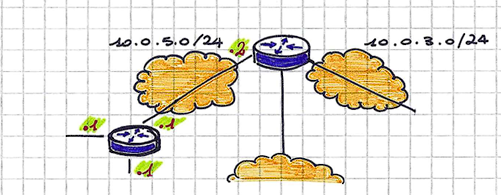
\includegraphics[width=0.8\linewidth]{Figures//05/interfacce.png}
    \caption{Dettaglio di un grafico di reti. Disegnato a mano da Yours Truly.}
    \label{fig:05interface}
\end{figure}

\newpage
\noindent La tabella di routing ha un aspetto del genere (stavolta fatta a mano perché è molto più carino spiegare ciascun campo così) (vedasi Fig. \ref{fig:routingtable}):

\begin{figure} [h]
    \centering
    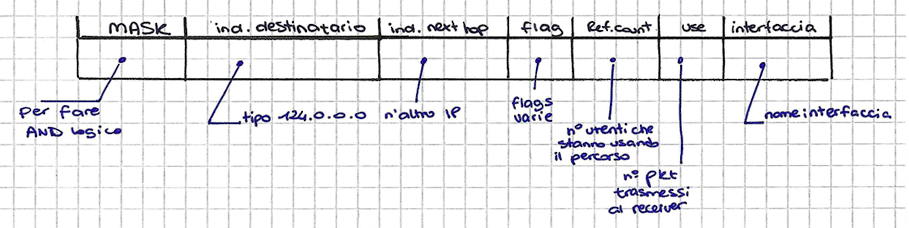
\includegraphics[width=1\linewidth]{Figures//05/routingtable.png}
    \caption{Dettaglio di un record di una tabella di routing. Di nuovo, cortesia di Yours Truly.}
    \label{fig:routingtable}
\end{figure}

\addcontentsline{toc}{subsection}{ICMP}
\subsection*{ICMP}
\index{ICMP}
\underline{I}nternet \underline{C}ontrol \underline{M}essage \underline{P}rotocol\\
incluso nello stack TCP/IP, è richiesto per qualsiasi implementazione standard di IP.\\

\noindent Fondamentalmente viene usato da IP per inviare messaggi di errore (per farlo, ICMP usa a sua volta IP. Meta! :D).\\


\begin{table}[h]
\centering
\begin{tabular}{ccc}
\multicolumn{3}{c}{Header ICMP (32 bit)}                                                                                    \\ \hline
\multicolumn{1}{|c|}{type (8 bit)} & \multicolumn{1}{c|}{code (8 bit)} & \multicolumn{1}{c|}{ICMP header checksum (16 bit)} \\ \hline
\end{tabular}
\end{table}

\noindent \openapex type'' specifica il formato, è un valore numerico associato a qualche informazione (e.g.: `0' = echo reply; `4' = source quench; `5' = redirect); \openapex code'' specifica il tipo di errore; il checksum è, di nuovo, il complemento a 1 di informazioni dell'header (IP, credo).\\

\noindent I messaggi sono di 2 tipi, fondamentalmente: segnalazione errori e richiesta informazioni.\\

\noindent Quando si usa il comando ``ping''\index{ping}, quello che succede è che viene creato un pacchetto ICMP di tipo ``8'', la risposta che arriva è un pacchetto ICMP di tipo ``1''.\\

\noindent Un altro tipo di messaggio era quello del ``timestamp'', serviva ad ottenere data e ora esatta segnata da certi host: ora questo servizio non si usa più perché tutti gli host usano il protocollo NTP (Network Time Protocol)\index{NTP}, che sincronizza gli orologi di tutti gli host al mondo con un orologio di riferimento.\\

\noindent Come funziona il \hl{Traceroute}\index{traceroute}:
\begin{itemize}
    \item il primo pacchetto è un messaggio ICMP con un TTL settato a 1: arriva al router immediatamente confinante, al che il TTL viene decrementato a 0 che innesca un messaggio ICMP di errore per TTL giunto a termine;
    \item il pacchetto seguente è di nuovo un messaggio ICMP con TTL settato a $1+1=2$: arriva al router immediatamente dopo, e si ripete la cosa del messaggio di errore;
    \item il processo viene ripetuto iterativamente con TTL incrementali così, in modo da ottenere info da tutti i router nel percorso. Fatto il traceroute :D
\end{itemize}

\noindent Protocolli di Routing AS (Autonomous Systems)\footnote{ASBR (Autonomous System Border Router)\index{ASBR}, router che tra le altre cose deve avere un'istanza sia dei router interni alla rete che di quelli esterni.}:
\begin{itemize}
    \item Protocolli inter-AS (esterni): BGP;
    \item Protocolli intra-AS (interni):
    \begin{itemize}
        \item \hl{distance vector}\index{distance vector}:
        \begin{itemize}
            \item RIP, RIP2\index{RIP}\index{RIP2};
            \item IGRP, EIGRP\index{IGRP}\index{EIGRP};
        \end{itemize}
        \item \hl{link state}\index{link state}:
        \begin{itemize}
            \item OSPF, OSPF2\index{OSPF}\index{OSPF2};
            \item IS-IS;
        \end{itemize}
    \end{itemize}
\end{itemize}

\noindent È importante che si sappia bene la differenza tra protocolli distance vector e protocolli link state, perché hanno degli scopi diversi!! I distance vector servono a trovare il percorso migliore tra router dato il numero di hop, i link state servono a scoprire com'è fatta la rete! Con i link state scopriamo tutte le rotte disponibili, con i distance vector scegliamo quella ottimale. Uno è puramente esplorativo, uno concerne l'ottimizzazione.\\

\addcontentsline{toc}{section}{Distance Vector}
\section*{Protocolli Distance Vector}
\index{distance vector!protocolli}
\noindent Vengono utilizzati per trovare il \hl{percorso migliore} nella rete, considerando come unità di misura il numero di hop tra un router e l'altro.\\

\noindent Fondamentalmente, ogni $x$ secondi, il router invia ai suoi vicini la propria routing table.\index{routing!tabella}\\
\addcontentsline{toc}{subsection}{Algoritmo RIP}
\subsection*{Algoritmo RIP}
\index{RIP!algoritmo}
\noindent \underline{R}outing \underline{I}nformation \underline{P}rotocol\\

\noindent\textcolor{Blue}{Differenza tra RIP e RIP 2: RIP era classful, RIP2 invece usa maschera (quindi è classless).}

\begin{enumerate}
    \item Consideriamo un router che al momento ha una tabella di routing così fatta:

\begin{table}[ht]
\centering
\begin{tabular}{ccc}
\multicolumn{3}{c}{Routing Table}                                                                                                   \\ \hline
\multicolumn{1}{|c|}{\textit{rete raggiungibile}} & \multicolumn{1}{c|}{n. Hop necessari} & \multicolumn{1}{c|}{router di origine:} \\ \hline
\multicolumn{1}{|c|}{Rete 1}                      & \multicolumn{1}{c|}{7}                & \multicolumn{1}{c|}{A}                  \\ \hline
\multicolumn{1}{|c|}{Rete 2}                      & \multicolumn{1}{c|}{2}                & \multicolumn{1}{c|}{C}                  \\ \hline
\multicolumn{1}{|c|}{Rete 6}                      & \multicolumn{1}{c|}{8}                & \multicolumn{1}{c|}{F}                  \\ \hline
\multicolumn{1}{|c|}{Rete 8}                      & \multicolumn{1}{c|}{4}                & \multicolumn{1}{c|}{E}                  \\ \hline
\multicolumn{1}{|c|}{Rete 9}                      & \multicolumn{1}{c|}{4}                & \multicolumn{1}{c|}{F}                  \\ \hline
\end{tabular}
\end{table}


    
    \item Il router riceve un messaggo da un certo Router C contenente la tabella di routing di C:

    \begin{table}[ht]
    \centering
    \begin{tabular}{cc}
    \multicolumn{2}{c}{Routing Table di C}                                                    \\ \hline
\multicolumn{1}{|c|}{\textit{rete raggiungibile}} & \multicolumn{1}{c|}{n. Hop necessari} \\ \hline
\multicolumn{1}{|c|}{Rete 2}                      & \multicolumn{1}{c|}{4}                \\ \hline
\multicolumn{1}{|c|}{Rete 3}                      & \multicolumn{1}{c|}{8}                \\ \hline
\multicolumn{1}{|c|}{Rete 6}                      & \multicolumn{1}{c|}{4}                \\ \hline
\multicolumn{1}{|c|}{Rete 8}                      & \multicolumn{1}{c|}{3}                \\ \hline
\multicolumn{1}{|c|}{Rete 9}                      & \multicolumn{1}{c|}{5}                \\ \hline
\end{tabular}
\end{table}
\item Il router prende queste informazioni, aumenta subito di 1 tutti gli hop dal Router C (l'hop che stiamo incrementando è il passo che serve per andare da questo router al router C);

\item La tabella ricevuta e incrementata viene ora comparata con quella che il router ha già: \begin{itemize}
    \item se la prima ha meno hop per raggiungere qualche rete, aggiorno quel campo con quello di C;
    \item se alcuni campi non erano presenti, vengono aggiunti (ad esempio, attraverso il router C ora possiamo raggiungere Rete 3);
    \item se il numero di Hop è lo stesso, è indifferente se aggiorniamo il campo della nostra tabella o no;
    \item se il numero di Hop è maggiore di quello che ho in tabella, non aggiorno la tabella con la nuova informazione;
\end{itemize}

\begin{table}[ht]
\centering
\begin{tabular}{ccc}
\multicolumn{3}{c}{Routing Table aggiornata}                                                                                        \\ \hline
\multicolumn{1}{|c|}{\textit{rete raggiungibile}} & \multicolumn{1}{c|}{n. Hop necessari} & \multicolumn{1}{c|}{router di origine:} \\ \hline
\multicolumn{1}{|c|}{Rete 1}                      & \multicolumn{1}{c|}{7}                & \multicolumn{1}{c|}{A}                  \\ \hline
\multicolumn{1}{|c|}{Rete 2}                      & \multicolumn{1}{c|}{5}                & \multicolumn{1}{c|}{C}                  \\ \hline
\multicolumn{1}{|c|}{Rete 3}                      & \multicolumn{1}{c|}{9 (nuovo)}                & \multicolumn{1}{c|}{C}                  \\ \hline
\multicolumn{1}{|c|}{Rete 6}                      & \multicolumn{1}{c|}{5 (sostituito 8F)}                & \multicolumn{1}{c|}{C}                  \\ \hline
\multicolumn{1}{|c|}{Rete 8}                      & \multicolumn{1}{c|}{4 (uguale)}                & \multicolumn{1}{c|}{C ( oppure E)}                  \\ \hline
\multicolumn{1}{|c|}{Rete 9}                      & \multicolumn{1}{c|}{4 (non aggiornato, $6>4$)}                & \multicolumn{1}{c|}{F}                  \\ \hline
\end{tabular}
\caption{Tabella di routing aggiornata. Nota: il valore di Rete 2 era 2 e proveniente da C, ma è stato aggiornato perché ora da C si arriva a Rete 2 con 5 hop.}
\end{table}
\item e questo è RIP.
\end{enumerate}

\addcontentsline{toc}{section}{Algoritmi di Instradamento}
\section*{Algoritmi di Instradamento}\index{instradamento!algoritmi}
\noindent O quella che il prof chiamò: Breve Carrellata di Algoritmi di Instradamento.\\

\noindent Il compito del livello di rete è di trasportare i pacchetti da un indirizzo di origine a un indirizzo di destinazione, ma non spetta a protocolli come IP occuparsi di come questo avviene fatto nella rete - di questo si occupano i Router! Di quale percorso far fare ai dati.\\

\noindent Riguardo il Forwarding diretto: all'interno dello stesso mezzo fisico possono esserci più reti a livello logico (pensate al subnetting con netmask): è compito del router occuparsi dell'instradamento anche lì tra quelle reti. In casi del genere è preferibile utilizzare una sola mega-rete che corrisponde alla topologia fisica. In casi quali? Immagino pensassi a casi in cui si fa spesso comunicazione interna, piuttosto che attraverso internet, non lo so sinceramente.\\

\noindent Protocollo Routabile (instradabile)\index{protocollo!instradabile}\index{protocollo!routabile}: protocollo che può essere utilizzato per applicare algoritmi di routing. Routing e Forwarding, utilizzati insieme, sono necessari per l'operatività di una rete. Informazione fondamentale a tale scopo è la tabella di routing.\\

\noindent Su tutte le macchine in cui è operativa la stack TCP/IP, siano essi End System o Router etc., è presente una tabella di routing ed esiste almeno un protocollo di routing.\\

\noindent Ciascun host è sempre collegato ad un default router, detto anche default gateway\index{default gateway}, detto anche first-hop router, detto anche router di primo rilancio, che comunica con la rete esterna.\\

\noindent Now onto our carrellata:
\begin{itemize}
    \item algoritmo di routing: trovare il miglior percorso da punto A a punto B ($\approx$ con il minor costo, data una certa misura tipo il nr Hop);
    \item Teoria dei Grafi (concetto visto nel corso di Algoritmi, tra le altre cose):
    \begin{itemize}
        \item Grafo\index{grafo}: un Grafo $\mathcal{G}=(\mathcal{N},\mathcal{E})$ è un insieme di $\mathcal{N}$ nodi ed $\mathcal{E}$ archi (dove E sta per Edges);
        \item Ad ogni arco che va dal nodo $x$ al nodo $y$ (arco $(x,y)$) è associato un costo $c(x,y)$;
        \item se il grafo non è orientato, allora vale sempre che gli archi sono uguali sia che vengono attraversati da x verso y che viceversa. $c(x,y) = c(y,x)$;
        \item $y$ è adiacente (o vicino) ad $x$ se esiste un arco che li collega: $(x,y)\in \mathcal{E}$;
        \item il costo complessivo di un percorso è la somma dei costi degli archi che lo compongono:
        \[c(x_1,x_n) = c(x_1,x_2)+c(x_2, x_3) +...+c(x_{n-1}, x_n)\]
    \end{itemize}
    \item 2 categorie di algoritmi di instradamento:
    \begin{itemize}
        \item statici: basati su tabelle manuali, percorsi che cambiano raramente;
        \item dinamici: la topologia della rete, i percorsi e i costi possono cambiare per cui bisogna adeguarsi spesso ai cambiamenti (questo viene fatto in base a un certo timer);
    \end{itemize}
    \item gli algoritmi si possono suddividere anche in queste due categorie:
    \begin{itemize}
    \item sensibili al carico: a seconda del carico della rete, cambierà la metrica;
    \item insensibili al carico: sono quelli utilizzati per la maggior parte (RIP, OSPF, BGP...)
    \end{itemize}
    \item ci sono altre due categorie che si possono usare come criterio:
    \begin{itemize}
        \item globali ($\approx$ link state): utilizzano tutti gli algoritmi a disposizione per conoscere l'intera mappa della rete. Per fare ciò, fanno quello che si dice \openapex flooding'' della rete;
        \item decentralizzati ($\approx$ distance vector): non c'è una conoscenza \textit{globale} della rete, solo dei nodi immediatemente vicini (più eventualmente il default gateway, ogni router ha conoscenza di se stesso!).
    \end{itemize}
\end{itemize}

\newpage
\addcontentsline{toc}{subsection}{Principio Distance Vector}
\subsection*{Principio Distance Vector}
\index{distance vector!principio}
\begin{figure} [ht]
    \centering
    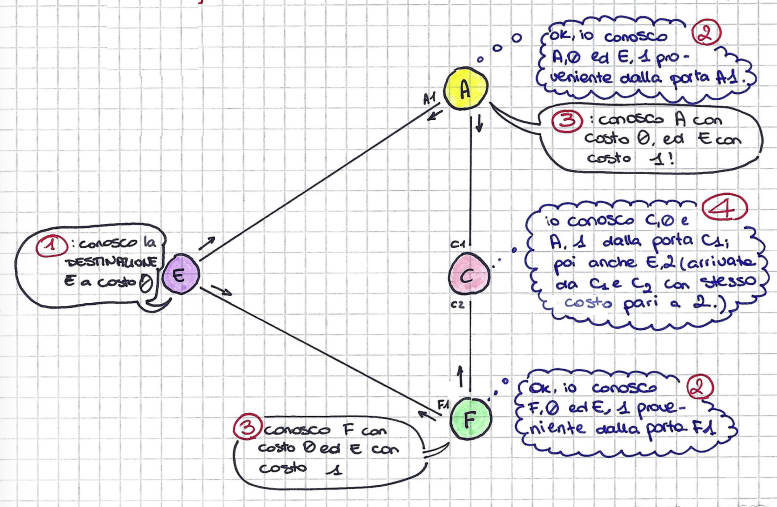
\includegraphics[width=0.8\linewidth]{Figures/05/distvec.png}
\end{figure}

\noindent Proprietà di:
\begin{itemize}
    \item distance vector:
    \begin{itemize}
        \item [+] semplici da implementare;
        \item [+] supportati da sistemi con scarse capacità di computazione e memoria;
        \item [-] problema del loop infinito (? anche se, stando alle mie note, questo è un problema che può essere risolto con il metodo ``split horizon''\footnote{vedere \href{https://www.techtarget.com/searchnetworking/definition/split-horizon}{qui :)}});
        \item [-] convergenza lenta (dipendente dal numero di nodi);
        \item [-] non possono usare molti hop (RIP ne ha massimo 15);
    \end{itemize}
    \item link state:
    \begin{itemize}
        \item [+] mappano la rete completamente;
        \item [+] non sono suscettibili a errori;
        \item [-] consumano moltissima banda (flooding);
        \item [-] non facilissimi da configurare;
        \item [-] richiedono capacità elevate in generale;
        \item [$\sim$] si usano in topologie dense di router.
    \end{itemize}
\end{itemize}

\noindent \textcolor{Blue}{La rete dell'università usa il protocollo link state OSPF.}\\

\noindent I pacchetti che il router invia per comunicare con gli altri le proprie informazioni si chiamano \openapex hello packet''.\\

\addcontentsline{toc}{section}{Algoritmi Link State}
\section*{Algoritmi Link State}
\index{link state!algoritmi}
\noindent Protocolli SSSP (Single Source Shortest Path):\begin{itemize}
    \item Algoritmo di Dijkstra;
    \item Algoritmo di Bellman-Ford;\footnote{differiscono essenzialmente per la metrica, se ho capito bene: il Bellman-Ford gestisce anche costi negativi, Dijkstra solo positivi.}
\end{itemize}
\addcontentsline{toc}{subsection}{Algoritmo di Dijkstra}
\subsection*{Alg. di Dijkstra}\index{Dijkstra!algoritmo}
\noindent L'algoritmo di Dijkstra si vede nel corso di Algoritmi, ragion per cui non lo approfondiremo troppo. Si consideri la rete in Fig. \ref{fig:dijkstra}, con i nodi che sono Router e gli archi che rappresentano il costo di ciascun collegamento:
\begin{figure} [ht]
    \centering
    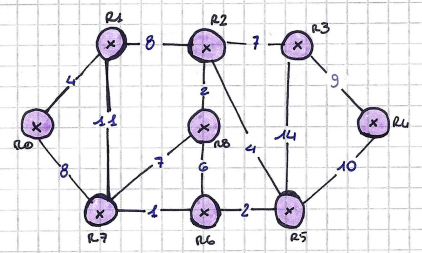
\includegraphics[width=0.75\linewidth]{Figures//05/dijkstra.png}
    \caption{Enter Caption}
    \label{fig:dijkstra}
\end{figure}

\begin{enumerate}
    \item Partiamo da $R_0$: i nodi che posso raggiungere e che scopro immediatamente sono $R_1$ con $c=4$ e $R_7$ con $c=8$;
    \item da $R_1$, $R_7$ posso scoprire $R_2$, $R_8$ e $R_6$;
    \item \textcolor{Red}{qual è il percorso meno costoso (che conosco ora) da $R_0$ a \{$R_2$, $R_8$, $R_6$\}}?
    \begin{enumerate}
        \item ($R_0\Rightarrow R_2$): $R_0\rightarrow R_1 \rightarrow R_2$ con costo $4+8=12$;
        \item ($R_0\Rightarrow R_8$): $R_0 \rightarrow R_1 \rightarrow R_2 \rightarrow R_8$ a costo $4+8+2=14$;
        \item ($R_0 \Rightarrow R_6$): $R_0\rightarrow R_7 \rightarrow R_6$ a costo $8+1=9$;
    \end{enumerate}
    \item da $R_2$, $R_8$, $R_6$ posso scoprire $R_3$ e $R_5$;
    \item \textcolor{Red}{qual è il percorso meno costoso (che conosco ora) da $R_0$ a \{$R_3, R_5$\}}?
    \begin{enumerate}
        \item ($R_0\Rightarrow R_3$): $R_0\rightarrow R_1 \rightarrow R_2 \rightarrow R_3$ a costo $4+8+7=19$;
        \item ($R_0 \Rightarrow R_5$): $R_0 \rightarrow R_2 \rightarrow R_6 \rightarrow R_5$ a costo $8+1+2=11$;
    \end{enumerate}
    \item infine, $R_0 \Rightarrow R_4$ si raggiunge via $R_0 \rightarrow R_7 \rightarrow R_6 \rightarrow R_5 \rightarrow R_4$ a costo $8+1+2+10=21$.
    \item Ci sono più percorsi possibili da $R_0$ ai vari router, ma questi che ho riportato sono i meno costosi!! Questo è ciò che ci interessa determinare. Tipo ($R_0\Rightarrow R_8$) passando per $R_0 \rightarrow R_1 \rightarrow R_7$, ma il costo sarebbe $4+11+7=22$;
\end{enumerate}

\begin{figure} [ht]
    \centering
    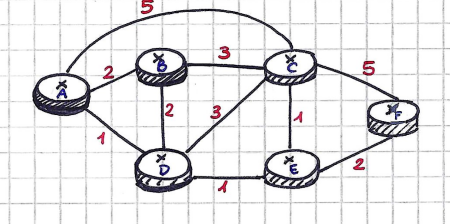
\includegraphics[width=0.75\linewidth]{Figures/05/dijkstra2.png}
    \caption{Altro esercizio da fare con Dijkstra.}
    \label{fig:dijk2}
\end{figure}

\noindent Al termine dell'esercizio proposto in Fig. \ref{fig:dijk2}, sperando che io non mi sia sbagliata, dovreste avere un risultato del genere:

\begin{table}[ht]
\centering
\begin{tabular}{|c|c|c|c|c|c|c|}
\hline
\textit{n. Hop da A} & Router attraversati & B   & C   & D   & E        & F        \\ \hline
0                    & A                   & 2,A & 5,A & 1,A & $\infty$ & $\infty$ \\
1                    & AD                  & 2,A & 4,D & -   & 2,D      & $\infty$ \\
2                    & ADE                 & 2,A & 3,E & -   & -        & 4,E      \\
3                    & ADEB                & -   & 3,E & -   & -        & 4,E      \\
4                    & ADEBC               & -   & -   & -   & -        & 4,E      \\
5                    & ADEBCF              & -   & -   & -   & -        & -        \\ \hline
\end{tabular}
\caption{Percorsi di minor costo da A alle varie direzioni.}
\end{table}

\begin{table}[ht]
\centering
\begin{tabular}{|c|c|c|}
\hline
\textit{destinazione} & next hop (passo 1) & costo \\ \hline
F                     & D                  & 4     \\
C                     & D                  & 3     \\
B                     & (B stesso)         & 2     \\
3                     & D                  & 2     \\
D                     & (D stesso)         & 1     \\ \hline
\end{tabular}
\caption{Tabella di Routing interna ad A.}
\end{table}


\addcontentsline{toc}{section}{Altro su Data Link e Ethernet}
\section*{Altre Cose su Data Link ed Ethernet}
\index{Ethernet}
\noindent In LAN, nel momento in cui un host trasmette nella rete, esso diventa proprietario di TUTTO il mezzo trasmissivo! (nel senso che, fintanto che è lui a parlare, è lui a monopolizzare il canale). Questo era un problema di sicurezza ``non indifferente'' agli albori della tecnologia LAN, il fatto che tutti i messaggi fossero broadcast, a cui si è in qualche modo ovviato con CSMA-CD, che vedremo in un attimo.\\
\noindent Con il termine Ethernet ci si riferisce sia alla tecnologia per connettere dispositivi in LAN (cablaggio e porte, immagino), sia ad una componente logica, algoritmica se vogliamo, utilizzata per gestire le trasmissioni di dati su questa rete. In altre parole, sentiamo parlare sia di ``Cavo Ethernet'' (tecnologia fisica) che di ``Frame Ethernet'' (tecnologia logica, come un Pacchetto IP).\\

\noindent Memo degli standard e di chi li ha pubblicati (cercate di ricordarveli questi, sono importanti):\index{standard!IEEE 802}
\begin{itemize}
    \item IEEE 802 : definisce diversi standard LAN, tra cui quelli più rilevanti sono:
    \begin{itemize}
        \item 802.3 : Ethernet;
        \item 802.11 : WLAN (Wireless LAN) \textit{\& Mesh (Wi-Fi certification)} (qualsiasi cosa significhi ciò);
        \item gli altri punti di IEEE 802 sono stati dismessi, come ad esempio 802.5 che definiva la topologia Token Ring (ampiamente in disuso oggi).
    \end{itemize}
    \item EIA/TIA 568\index{standard!EIA/TIA 568} : definisce gli standard per il cablaggio strutturato (e.g. come vanno disposti i cavi colorati all'interno della spina RJ-45 ad un estremo e all'altro del cavo Ethernet\index{Ethernet!cavo}, se si vogliono creare cavi Straight-Through o Crossover, questo lo vedremo nel prossimo capitolo);
\end{itemize}

\noindent Di nuovo, giusto per ripetermi: a livello Data Link, la PDU prende il nome di Trama o Frame (quindi per esempio si parla di ``Frame'' Ethernet).\\
\index{Ethernet!frame}
\noindent La struttura del Frame Data Link dipende dalla tecnologia fisica sottostante, pertanto non c'è uno standard unico ben preciso sulla struttura di un Frame. In linea generica, però, le sue dimensioni sono comprese tra $64\div 1518$ Bytes, e tra le informazioni trasmesse ci sono:
\begin{itemize}
    \item un trailer all'inizio, che contiene indirizzi di destinatario e mittente;
    \item il payload;
    \item una forma di rilevazione errori come CRC\index{CRC}, controllo a ridondanza ciclica, o controllo di parità i somme di controllo;
\end{itemize}

\noindent I collegamenti possono essere fondamentalmente di 2 tipi:
\begin{itemize}
    \item Broadcast : più stazioni connesse con lo stesso mezzo trasmissivo;
    \item Point to Point : cablato o wireless, collega una stazione ad una stazione e basta. (in casi come questo viene utilizzato il cavo Cross-Over, e più in generale ogniqualvolta si intende collegare tra loro due dispositivi dello stesso tipo, Router a Router, Host a Host...)
\end{itemize}

\noindent In caso di reti ad accesso multiplo (LAN, reti via satellite...), sono richiesti protocollo ad accesso multiplo per dirigere il traffico senza causare collisioni\index{collisioni}. Questi possono operare per:
\begin{itemize}
    \item suddivisione del canale in TDM/FDM (come dicevamo nell'introduzione, dividere la banda comune in slot di tempo o di frequenza) ($\approx$ Channel Partitioning Protocols);
    \item accesso casuale (RAP, Random Access Protocols), come lo Slotted ALOHA;
    \item a rotazione (taking-turn protocols), in cui gli host parlano a turno secondo diversi criteri come Polling o Token-Passing. 
\end{itemize}

\noindent Tecniche di allocazione del canale trasmissivo:
\begin{itemize}
    \item statica: il mezzo viene partizionato tipo TDM/FDM;
    \item dinamica: tutte le frequenze del mezzo trasmissivo vengono assegnate di volta in volta ai vari host (nel caso dei protocolli turn-based, naturalmente, occorre definire un algoritmo che gestisca questa assegnazione dinamica).
\end{itemize}

\newpage
\noindent Sketch originale\index{Ethernet!tecnologia} (riprodotto da me, ofc) della tecnologia Ethernet, ideata nel 1976 da Metcalfe:\\
\begin{wrapfigure}{l}{0.6\textwidth}
 \begin{center}
 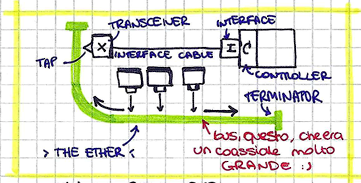
\includegraphics[width=1\linewidth]{Figures/05/ethernet1976.png}
  \end{center}
  \label{fig:eth1976}
\end{wrapfigure}

\begin{itemize}
    \item c'è un solo bus condiviso (in origine, un cavo coassiale);
    \item  è non-deterministico - non c'è nessuna regola che stabilisce quando parla chi (quindi ci si chiede: quando e dove si trasmette sul bus?)
    \item ad oggi, Ethernet è la tecnologia cablata più diffusa, si è passati da una topologia a Bus come quella nello sketch ad una topologia a stella (switched Ethernet\footnote{vedremo poi che si è passati all'utilizzo del cosiddetto Ethernet Hub, che comunque contiente una forma di Bus al suo interno})
\end{itemize}

\noindent Topologia a Bus:\index{topologia!a bus}
\begin{itemize}
    \item 
interruzione del bus in qualsiasi punto $\rightarrow$ interruzione di tutta la rete;
\item aggiungere un end system alla rete comporta un grosso intervento, con interruzione del servizio nell'intero sistema;
\item un frame immesso nel bus si propaga ogni volta in entrambe le direzioni del bus.
\end{itemize}

\noindent Aloha\index{Aloha}: protocollo per topologie a Bus (indovinate in che paese è stato ideato). Consente trasmissione in modo casuale, quindi spesso i frame mandati in rete allo stesso momento andavano in collisione! Collisioni che potevano essere parziali o totali, a seconda della \% di timeslot sovrapposti tra i messaggi in conflitto. È un protocollo facile da realizzare, ma naturalmente presenta dei problemi di efficienza.

\addcontentsline{toc}{subsection}{CSMA: Gestione Collisioni}
\subsection*{CSMA}\index{collisioni!CSMA}
\noindent \underline{C}arrier \underline{S}ense \underline{M}ultiple \underline{A}ccess, dove Carrier Sense è un modo per dire, più o meno: ``prima di parlare, ascolta.'' (e mentre trasmetti, continua ad ascoltare)

\begin{itemize}
    \item CSMA-CA: Collision Avoidance;
    \item CSMA-CD: Collision Detection.
\end{itemize}

\noindent Ma! Neppure l'utilizzo dei protocolli CSMA-CA/CD scongiura del tutto le collisioni.\\
\noindent Supponete che per caso inizino a parlare 2 End Systems in contemporanea: collidono una volta, si fermano entrambi e lasciano parlare l'altro, tipo la scena cliché in cui due persone iniziano a dire entrambe ``no scusa, vai prima tu'' e così facendo parlano assieme di nuovo e avanti così più e più volte.\\
\noindent Come si scongiura questa situazione di stallo infinito deadlock? Si tenta di dire, al momento della collisione, agli host di aspettare un tempo $T$ generato randomicamente: questa istruzione di aspettare viene data attraverso un segnale speciale (``jamming'') che ha una certa frequenza;\\
\noindent Se, disgraziatamente, i tempi randomici scelti dalle parti coinvolte sono di nuovo uguali e c'è di nuovo interferenza, si raddoppia il range di tempi T di attesa da scegliere a caso! Nel senso: se alla prima collisione avrei aspettato un tempo nell'insieme I$\mathcal{T}=\{0,1\}$, la seconda volta sceglierò tra $\mathcal{T}' = \{0,1,2,3\}$: più elementi ci sono nell'insieme $\mathcal{T}$, minore è la probabilità che 2 End System peschino lo stesso $t$. Questo meccanismo si chiama ``Exponential Backoff''.\index{collisioni!exponential backoff}\\

\noindent Andiamo avanti. Dominio:\index{dominio}
\begin{itemize}
    \item di Broadcast: parti di rete in cui il messaggio broadcast riesce a raggiungere tutti gli host: nel caso di una LAN, il dominio di BC e limitato dal Router (Gateway).
    \item di Collisione: parti della rete dove c'è la possibilità che si verifichino collisioni.
\end{itemize}

\noindent Tempo per rilevare una collisione:
\[a = \dfrac{\text{lunghezza\_collegamento}}{\text{lunghezza\_pkt}}\]
\newpage
\addcontentsline{toc}{chapter}{Physical Layer e Sicurezza}
\chapter*{\begin{center}\texttt{6 - Livello Fisico e Sicurezza}\end{center}}
\hrulefill \\
\addcontentsline{toc}{section}{Specifiche Ethernet}
\section*{Specifiche fisiche Ethernet}
\index{Ethernet!specifiche fisiche}
\begin{itemize}
    \item 10BaseT, dove 10 è la banda base, T sta per ``Twisted Pair''.
    \begin{itemize}
        \item trasmissione 10mbps in banda base;
        \item sia coassiale che UTP (la cronologia dei cambiamenti nella tecnologia ha fatto: coassiale thick $>$ coassiale thin $>$ doppino CAT3);
        \item lunghezza max cavo: 100 metri;
        \item connettore RJ45, affidabile ed economico, facile da implementare, al contrario del BNC che unisce i coassiali.
    \end{itemize}
    \item 100BaseT, differisce da 10BaseT in:
    \begin{itemize}
        \item la velocità di trasmissione;
        \item ha 3 tipi possibili di connettore:
        \begin{itemize}
            \item 100Base-T4, doppino 4 coppie;
            \item 100Base-TX, doppino 2 coppie;
            \item 100Base-FX, fibra ottica.
        \end{itemize}      
        \item comunque è retrocompatibile con 10BaseT;
    \end{itemize}
    \item Gigabit Ethernet (802.3Z): fino  1Gbps e non retrocompatibile.
    \item Questi standard Ethernet sono tutti a tecnologia CSMA-CD  
\end{itemize}

\noindent Topologia ad Anello:\index{topologia!ad anello}
\begin{figure} [ht]
    \centering
    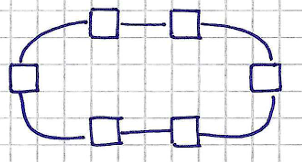
\includegraphics[width=0.5\linewidth]{Figures/06/ringtop.png}
    \caption{Topologia ad anello, supersemplificata.}
    \label{fig:06tknrng}
\end{figure}

\begin{itemize}
    \item semplifica coordinamento accessi;
    \item più facile identificare guasti;
    \item se si guasta un solo elemento, la rete è persa (come i circuiti in serie contrapposti a quelli in parallelo, non so se avete presente il discorso fondamentale dei circuiti elettrici)
\end{itemize}
\noindent Tecnologia ``Token Ring''\index{token ring}: dove il Token è un tipo particolare di frame che dà il permesso agli host per parlare. In Ethernet non c'è modo di stabilire chi può parlare quando. Sul piano Logico, le Token Ring sono disposte ad anello (vedasi Fig. \ref{fig:06tknrng}), ma Fisicamente conviene disporle come stella a doppio anello e utilizzare un MAU, Media/Multistation Access Unit.\\
\noindent Topologia FDDI: Fiber Distributed Data Interface (in disuso),\index{topologia!FDDI} sempre di tipo Token Ring, sempre cablata ad anello o stella, viaggiava a velocità elevate. Usava il doppio anello, due anelli indipendenti (rete autoriparante!).\\

\addcontentsline{toc}{section}{Wireless}
\section*{Livello fisico, reti wireless}
\index{rete, wireless}
\noindent Utilizzano \index{standard!IEEE 802.11}(standard IEEE 802.11\footnote{802.11a : standard per la rete 5 GHz, 802.11b/g : 2.4GHz (802.11b ha max vel. 11Mbps, 802.11g ha max vel. 54Mbps}): \begin{itemize}
    \item radiofrequenze;
    \item infrarossi.
\end{itemize}
\noindent Devono avere un access point\index{access point} collegato alla rete cablata;\\
\noindent L'arbitraggio\index{arbitraggio} del canale trasmissivo si può fare attraverso vari algoritmi (non c'è uno standard preciso);\\
\noindent Velocità di trasmissione: fino a 300Mbps;\\
\noindent Alcune problematiche del caso:\begin{itemize}
    \item propagazione onde radio;
    \item occupazione delle frequenze;
    \item inaffidabilità;
    \item potenza ridotta;
    \item sicurezza.
\end{itemize}
\noindent Più l'host è distante dall'access point, meno sarà la velocità di navigazione (max 50mt circa).\\

\noindent Tipi di interferenze:\index{interferenze}
\begin{itemize}
    \item strutturali: in edifici di cemento armato, la propagazione del segnale è difficile;
    \item su distanze elevate (e.g. ponti radio): edifici, vegetazione, nebbia e fenomeni atmosferici possono disturbare il segnale, le antenne vanno posizionate in un punto adeguato;
    \item dovute ad altre sorgenti: Bluetooth, interfoni per neonati, molti apparecchi utilizzano la frequenza $f = 2.4 GHz$ (con la 5 GHz si verificano meno interferenze).
\end{itemize}

\noindent Modalità di collegamento:
\begin{itemize}
    \item Peer to Peer (P2P): senza passare per l'access point\footnote{Penso che il Peer to Peer in internet sia diverso dal Peer to Peer che si intende qui. Qui penso si intenda una connessione fisica come quella che potremmo fare tra due PC sulla stessa scrivania, magari con tecnologia Bluetooth}. Dipende dalla scheda di rete del dispositivo;
    \item Client - Access Point;
    \item Multiple Access Point \& Roaming. mobilità: l'utente cambia access point mentre si sposta, senza percepire interruzioni di servizio;
    \item Bridging con antenna direzionale
\end{itemize}
\noindent Area di servizio: l'ambito in cui interviene l'access point.\\

\addcontentsline{toc}{subsection}{Sicurezza Wireless}
\subsection*{Sicurezza - Wireless}
\noindent Livelli di sicurezza Wireless:\index{wireless!sicurezza}
\begin{itemize}
    \item open system: detto anche ``con chiave di autenticazione condivisa'', non è esattamente la stessa cosa che dire ``possono entrare tutti''. Vuol dire che è aperta, sì, ma non sono necessariamente la stessa cosa;
    \item WEP: Wired Equivalent Privacy;\index{WEP}
    \item WPA/WPA2: WiFi Protected Access. Queste offrono:\index{WPA/WPA2}
    \begin{itemize}
        \item cifratura dei dati (standard IEEE 802.1X);
        \item integrità dei dati (garanzia che i dati ricevuti sono uguali a quelli spediti, nessuno li ha manomessi lungo il tragitto);
        \item protezione da attacchi Replay\footnote{attacco Replay: catturare pacchetti scambiati tra client e server e replicarli facendoli partire dall'indirizzo dell'attaccante allo scopo di risalire a chiavi di autenticazione.}
    \end{itemize}
\end{itemize}

\noindent WPA:
\begin{itemize}
    \item Personal: privata;
    \item Enterprise: ha bisogno di un Server di Autenticazione (e.g.: Radius, TACACS) che contiene cose come le credenziali degli utenti; 
\end{itemize}

\addcontentsline{toc}{subsection}{Wireless Sensor Network}
\subsection*{Wireless Sensor Network}\index{wireless!sensor network}
\noindent Reti di sensori collegate a controllori come Arduino. I sensori sono dispositivi piccoli, economici, limitati in capacità di elaborazione e trasmissione. Fondamentalmente rilevano delle misurazioni: di luminosità, di temperatura, di umidità, etc.\\
\noindent Caratteristiche delle reti di sensori:
\begin{itemize}
    \item composte da molti sensori che monitorano fenomeni in continuazione;
    \item reti Ad-Hoc, disegnate su misura per ciascuna situazione;
    \item dialogano tra loro tramite antenna;
    \item convergono tutti con i propri dati nel Sink (server centrale);
    \item ZigBee: standard (802.15.4) RL-WPAN, Wireless Personal Area Network; opera su frequenza 2.4 GHz a basso consumo.\index{standard!ZigBee}
\end{itemize}



\begin{wrapfigure}{r}{0.5\textwidth}
 \begin{center}
 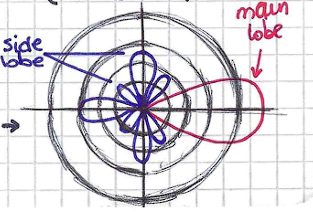
\includegraphics[width=1\linewidth]{Figures/06/onde.png}
    \caption{Diagramma di radiazione supersemplificato}
    \label{fig:06diag}
  \end{center}
\end{wrapfigure}

\noindent Propagazione delle onde:\\
\noindent Potenza di radiazione: la normativa tecnica ETS 300-328 impone di NON irradiare con una potenza EIRP\footnote{Effective Isotropic Radiated Power} $> 100 \text{mW (}\approx 20\text{dBm)}$.\\

\noindent Propagazione:\begin{itemize}
    \item Direzionale: guadagno $>1$;
    \item Omnidirezionale: guadagno $=1$.
\end{itemize}

\noindent Ogni antenna ha il suo diagramma di radiazione per aiutare a capire come orientarla al meglio (sketch in Fig. \ref{fig:06diag}).\\

\noindent Grado di protezione IP\index{IP (Ingress Protection)}(Ingress Protection), indicatore del grado di protezione di un dispositivo da agenti esterni. Formato da 2 cifre:
\begin{itemize}
    \item [I.] (Valore $0\div6$): protezione da oggetti solidi (dove 0 corrisponde a ``nessuna protezione'' e 6 corrisponde a ``protezione totale da polveri'');
    \item [II.] (Valore $0\div8$): permeabilità dell'acqua (dove 0 corrisponde a ``nessuna protezione'' e 8 corrisponde a ``resistente a immersione continua'')
\end{itemize}

\addcontentsline{toc}{section}{Altre specifiche dello Standard 802.3}
\section*{Altre specifiche dello Standard 802.3}\index{standard!IEEE 802.3}
\noindent Ovvero, altro cablaggio.\\

\addcontentsline{toc}{subsection}{Coassiali e Doppini Intrecciati}
\subsection*{Coassiale e Doppino Intrecciato}\index{cavo coassiale}
\begin{itemize}
    \item 10Base5: definisce il cosiddetto ``coassiale thick'' (lunghezza fino a 500m)
    \begin{itemize}
        \item ``thicknet'':\index{cavo coassiale!thicknet} consisteva in un unico bus coassiale, ciascuna macchina per collegarsi al bus aveva bisogno di un Transceiver (costoso, ndr)\index{transceiver}. Sulle schede di rete, per collegarsi al Transceiver, c'era una interfaccia AUI come quella in Fig. \ref{fig:06thicknet}
    \end{itemize}
    \item 10Base2: ovvero, il ``coassiale thin''\index{thinnet} (lunghezza fino a 185m). Nella ``thinnet'' non c'era più bisogno del Transceiver, in compenso però non si potevano usare prolunghe. L'interfaccia usata si chiama comunemente ``T'' (Fig. \ref{fig:06T})
\end{itemize}

\begin{figure} [ht]
    \centering
    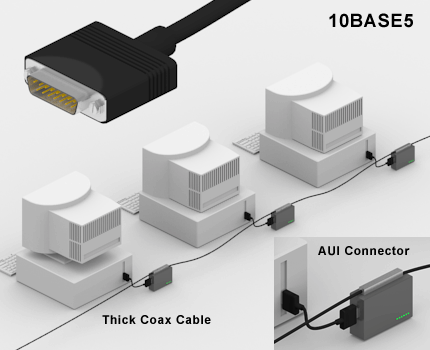
\includegraphics[width=0.6\linewidth]{Figures//06/thicknet.png}
    \caption{Rappresentazione di rete Thicknet. Fonte: \href{https://www.computerlanguage.com/results.php?definition=thick+Ethernet}{ComputerLanguage.com}}
    \label{fig:06thicknet}
\end{figure}
\begin{figure} [ht]
    \centering
    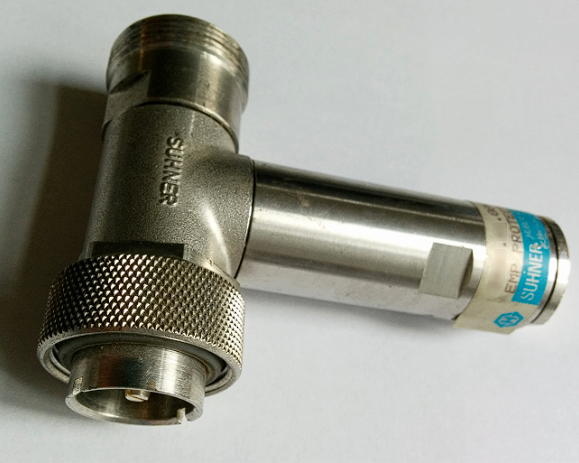
\includegraphics[width=0.5\linewidth]{Figures/06/Tconn.png}
    \caption{Connettore T per reti Thinnet. All'estremità ``lunga'' viene collegato il terminale, a quelle corte rispettivamente l'input e il resto del ring (o un Terminatore, tipo un tappo a impedenza $50\Omega$ di tipo BNC come le altre estremità dei coassiali)}
    \label{fig:06T}
\end{figure}

\noindent Doppino telefonico:\index{doppino}
\begin{itemize}
    \item non ci si collega più ad un bus comune ma a degli Switch;
    \item connettori BNC sostituiti da connettori RJ45;
    \item max distanza 100m.
\end{itemize}

\noindent La disposizione dei fili all'interno del connettore RJ45\index{RJ45} determina che tipo di collegamento si sta creando (schema T568-A, T568-B, in Fig. \ref{fig:06RJ45}):
\begin{itemize}
    \item se si realizza un cavo con connettori uguali a entrambe le estremità (quindi A-A o B-B), il cavo sarà di tipo straight-through;
    \item se si configurano connettori diversi (A-B, B-A), il cavo esce di tipo cross-over;
\end{itemize}

\begin{figure} [ht]
    \centering
    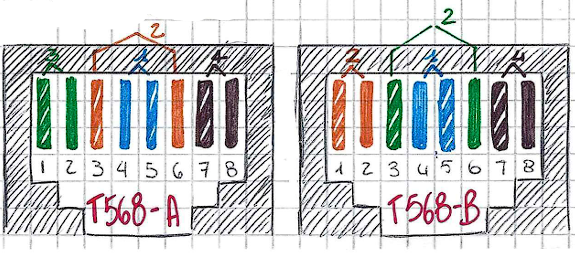
\includegraphics[width=0.75\linewidth]{Figures//06/rj45ab.png}
    \caption{Schema delle binature T568-A e T568-B.}
    \label{fig:06RJ45}
\end{figure}

\noindent Doppini:\index{doppino}\index{T568-A, T568-B}
\begin{itemize}
    \item UTP: doppino non-schermato (Unshielded Twisted Pair);\index{UTP}
    \item FTP: doppino schermato con foglio di alluminio + collegamento a massa (Foiled Twisted Pair);
    \item STP: doppino con schermo locale (Shielded Twisted Pair);
    \item S-UTP / S-FTP: doppino con schermo locale e foglio di alluminio.
\end{itemize}


\newpage
\noindent Categorie:\index{doppino!CAT}
\begin{itemize}
    \item [CAT 1]: solo per segnali vocali (telefonia);
    \item [CAT 2]: max vel. 4Mbps;
    \item [CAT 3]: max vel. 10Mbps;
    \item [CAT 4]: max vel. 16Mbps;
    \item [CAT 5]: max vel. 100Mbps con banda passante 100MHz;
    \item [CAT 5e]: max vel. fino a 1Gbps;
    \item [CAT 6]: max vel. fino a 10Gbps, banda passante fino a 250MHz;
    \item [CAT 7]: non riconosciuto da EIA/TIA.
\end{itemize}
\noindent N.B.: queste note sono state redatte inizialmente nel 2021, quindi non sono da escludere nuovi sviluppi di standard del doppino. Per preservare l'intreccio dei cavi interni, le norme di installazione vogliono che non si eserciti una forza superiore a $11,3$ Kg (insomma, non tirare i cavi così forte).\\

\addcontentsline{toc}{subsection}{Fibra Ottica}
\subsection*{Fibra Ottica}
\index{fibra ottica}
\begin{figure} [ht]
    \centering
    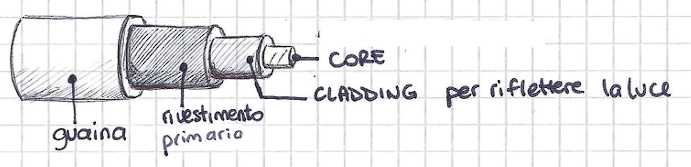
\includegraphics[width=0.75\linewidth]{Figures//06/of.png}
    \caption{Schema della struttura interna di un cavo di fibra ottica.}
    \label{fig:06OF}
\end{figure}\index{fibra ottica!cavo}
\begin{itemize}
    \item la fibra ottica, al contrario del coassiale e del doppino (che hanno bisogno di tutte quelle schermature) è immune alle interferenze;
    \item può essere:
    \begin{itemize}
        \item monomodale;
        \item multimodale (trasmette luce su più frequenze);
    \end{itemize}
    \item  tipo di connettore: ST (Straight Tip), o più spesso SC (Standard Connector).
\end{itemize}

\addcontentsline{toc}{section}{Estensione di una LAN}
\section*{Estensione di una LAN}\index{LAN!estensione}
\noindent Perché estendere una LAN?
\begin{itemize}
    \item unificare LAN costruite in momenti diversi;
    \item unificare LAN situate in diversi edifici; 
    \item distribuire carichi di traffico elevati;
    \item aumentare la distanza copribile;
    \item aumentare l'affidabilità;
    \item aumentare la sicurezza.
\end{itemize}
\noindent Ci sono naturalmente delle limitazioni dovute a protocolli di accesso e al decadimento del segnale - non si può espandere all'infinito, insomma.\\
\noindent Come estendere una LAN?
\begin{itemize}
    \item con dei Repeater\index{repeater} (Layer 1 device): come un buffer di segnale;
    \item  con dei Bridge\index{bridge} (Layer 2 device): leggono l'intestazione dei frame e inoltrano in base al contenuto che leggono. Non propagano collisioni. Sono adattivi, ovvero si configurano a mano a mano che ricevono informazioni sulla rete (credo facciano similmente agli switch). È possibile collegare con un bridge anche reti con tecnologie diverse, ad esempio Ethernet con Token Ring.
\end{itemize}

\begin{figure} [ht]
    \centering
    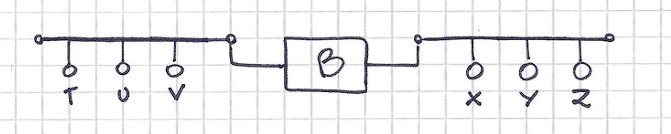
\includegraphics[width=0.75\linewidth]{Figures//06/bridge.png}
    \caption{Bridge B collega due LAN di host TUV e XYZ.}
    \label{fig:06bridge}
\end{figure}

\begin{itemize}
    \item Transparent Bridge: se X deve comunicare con Z nell'esempio in Fig. \ref{fig:06bridge}, la prima volta il frame viene inoltrato lungo TUTTA la rete, ma al ritorno il bridge avrà già appreso che X e Z sono nella stessa porzione di rete, quindi eviterà di inoltrarlo alla parte con TUV. (Backward Learning)
    \item Source Node Bridge: i bridge non mantengono queste informazioni di routing, ma sono capaci di selezionare il percorso ottimale tra due punti.
\end{itemize}
\noindent Ciclo di Bridge: dovuto a flooding, alcuni frame rimangono in circolo a lungo senza raggiungere una destinazione. Soluzione: Distributed Spanning Tree Protocol (STP), serve per far comunicare i bridge, in breve.\\

\addcontentsline{toc}{subsection}{Fault Tolerance}
\subsection*{Fault Tolerance}\index{fault tolerance}
\begin{figure}
    \centering
    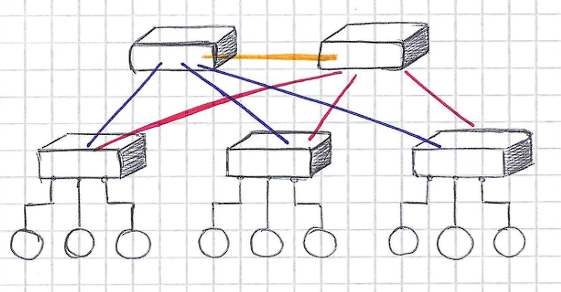
\includegraphics[width=0.75\linewidth]{Figures/06/ft.png}
    \caption{Centro Stella Ridondato, meccanismo di fault tolerance}
    \label{fig:06csr}
\end{figure}
\noindent Si costruisce una rete con doppi concentratori (Fig. \ref{fig:06csr}), in modo tale che se uno dovesse smettere di funzionare, l'altro terrebbe comunque in normale funzione il servizio. Aggiungere dispositivi ``di scorta'' prende il nome di Ridondanza.\\
\noindent Gli switch possono essere stackati (ad esempio, se ne può creare uno a 96 porte impilandone 2 da 48). Gli switch si possono gestire con CLI o GUI, accessibili via cavo o remote shell.\\ 
\noindent La tecnologia VLAN (Virtual LAN)\index{LAN!virtuale(VLAN)} serve a dividere virtualmente un solo switch in più LAN.\\
\noindent Reti Commutate (con Switch) $\approx$ come un mega bridge, in un certo senso. Lavorano in 3 modalità:\index{rete!commutata}
\begin{itemize}
    \item Cut-Through: lo switch legge il MAC, inoltra dove deve, fine.
    \item Store \& Forward: Legge il MAC, immagazzina tutto il messaggio e ne controlla i CRC, inoltra se tutto ok;
    \item Fragment Free: una via di mezzo, legge solo i primi 64 Byte del frame e fa controlli solo su quel prefisso. Se tutto ok, inoltra. (tant'è che, a differenza del header IP, nello header MAC viene prima il campo Destinazione poi Sorgente)
\end{itemize}
\newpage
\addcontentsline{toc}{chapter}{Note di Laboratorio 2024}
\chapter*{\begin{center}\texttt{Note di Laboratorio 2024\\a cura di Frascott}\end{center}} %aggiungi il tuo nome, o le iniziali, o uno pseudonimo, come vuoi 
\hrulefill \\

TBA
% @fra, questo è il tuo playground. Io sono stata educata a non usare i doppi backslash per andare a capo, e a indentare sempre, motivo per cui ora uso un sacco di doppi backslash e non indento un cazzo - perché mi piace di più così e i miei documenti LaTeX li formatto come diavolo mi pare, cheers <3

% forse quando sarai una cima in materia mi additerai come un'eretica, ma come tutti gli eretici morirò al rogo senza rimangiarmi la mia opinione. B) detto ciò, divertiti qui, puoi anche scrivere tutto come se fosse un file .txt, poi lo formattiamo insieme. Ottima cosa sviluppare un po' di soft skill con LaTeX, che poi è tipo HTML alla fine. Così scriverai una tesi spaziale a fine percorso. :D HF!!

%ctrl + Enter per compilare, se ti serve qualcosa scrivimi quando ti pare

% cleo xx

%p.s. hai anche una cartella per le immagini, se le vuoi annettere. è in Figures>lab-cheatsheet, meglio tenere le immagini ordinate in cartelle sennò si diventa scemi. Non farti scoraggiare dalla formattazione di immagini tabelle etc., non è difficile come sembra. D'altronde, se ce la faccio io... e.e

\addcontentsline{toc}{section}{Virtual Machines}
\section*{Virtual Machines}







%\newpage
\printindex
\end{document}

